\chapter{The CMS Experiment at the LHC}
\label{sec:cms}

\section{The Large Hadron Collider}
\label{sec:cms:lhc}.

The Large Hadron Collider (LHC)~\cite{lhcjinst}\footnote{Unless otherwise specified, all technical specifications of the LHC are derived from Reference~\cite{lhcjinst}} is a circular particle accelerator, 27 km in circumference and between 40 and 175 m below the surface. 
The ring cross the French-Swiss border near the city of Geneva. 
Designed to collide protons at a maximum center-of-mass energy $\sqrt{s} = 14$ TeV, the LHC has delivered collisions at $\sqrt{s}=7,8$ TeV (Run 1) and $\sqrt{s} = 13$ TeV (Run 2); the target energy $\sqrt{s} = 14$ TeV will be reached in Run 3. 
In addition to protons, the LHC accelerates and collides heavy nuclei (Pb and Xe) at lower values of $\sqrt{s}$. 
In this thesis, we focus exclusively on data recorded from proton collisions during Run 2. 

\begin{figure}[]
    \begin{center}
        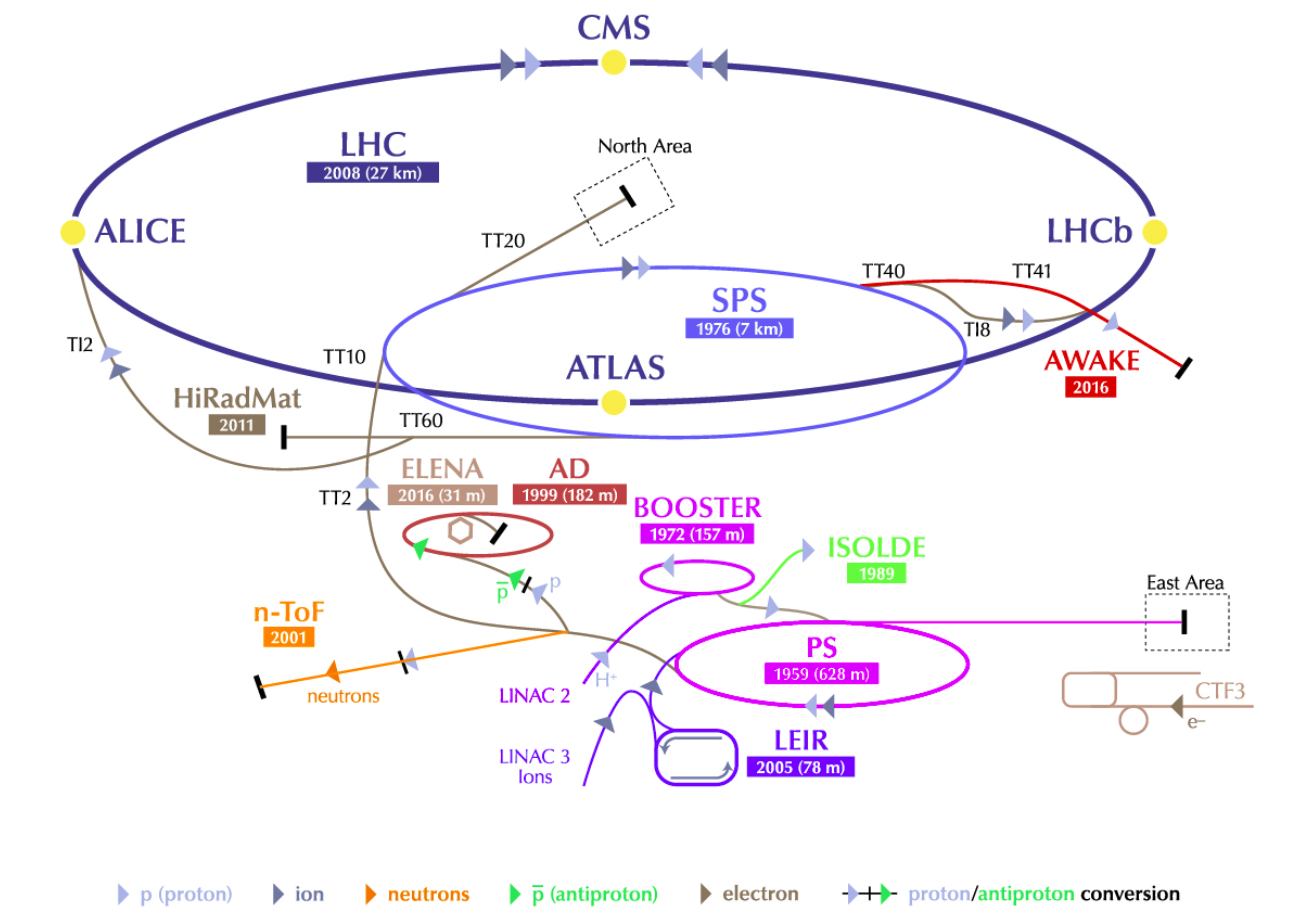
\includegraphics[width=0.8\textwidth]{figures/cms/lhc.png}
        \caption{Diagram of the CERN accelerator complex.
                 The LHC (dark blue) is fed protons (and heavy ions) by a chain of intermediate accelerators, beginning with LINAC2 (dark pink).i
                 Reprinted from Reference~\cite{lhcpic}. 
                    }
        \label{fig:cms:lhc}
    \end{center}
\end{figure}

Protons are brought to the LHC by the multi-stage process~\cite{lhctdr3} depicted in Figure~\ref{fig:cms:lhc}.
Hydrogen atoms are stripped of electrons and accelerated to a kinetic energy of $50$ MeV by LINAC2, a linear accelerator.
Subsequently, the Booster ring, the Proton Synchrotron (PS) and Super Proton Synchrotron (SPS) successively accelerate the protons to energies of 1.4, 26, and 450 GeV, respectively. 
Protons exit the SPS and enter the LHC at one of two places, corresponding to two different beams traveling in opposite directions.
The two beams intersect in eight places along the LHC, four of which are instrumented by a detector experiment: CMS, ATLAS, LHCb, and ALICE. 

Each proton beam in the LHC is accelerated by eight superconducting cavities exerting 400 MHz oscillating electric fields parallel to the beam line (the \emph{longitudinal} direction).
The maximum RF voltage seen by each beam is 16 MV per revolution.
The physical and temporal design of the RF system creates bunches of protons, corresponding to nodes of the oscillating field, approximately 7.5 cm in length and separated by 25 ns. 
Superconducting NbTi dipole magnets bend the two proton beams in opposite directions as they travel around the ring. 
Each of the 1232 dipoles is 14 m long and exerts a transverse $B$ field between $0.54$ and $8.33$ T.
To achieve such high $B$ fields, the magnets are cooled to 2 K by superfluid helium.
In addition, a number of quadrupole magnets are used to focus and match the beams between the dipoles\footnote{Full details on the various quadrupoles can be found in Table 3.7 of Reference~\cite{lhcjinst}.}.

The two main figures of merit for a collider the center-of-mass energy $\sqrt{s}$ and the number of events produced per unit time.
The latter is defined as:
\begin{equation} 
    N(pp\rightarrow X) = \int \di t~ L \sigma(pp\rightarrow X)
\end{equation}
where $\sigma$ is the cross section of the relevant process and $L$ is the instantaneous luminosity of the LHC. 
The cross section is fixed by nature, and so increasing the luminosity is the only handle to increase $N$. 
The instantaneous luminosity of two Gaussian beams is given by~\cite{lhcjinst}:
\begin{equation}
    L = \frac{N_b^2 n_b f_\mathrm{rev} \gamma F}{4\pi\epsilon \beta^*}
\end{equation}
where:
\begin{itemize}
    \setlength\itemsep{1pt}
    \item $N_b$ $=$ particles per bunch
    \item $n_b$ $=$ bunches per beam 
    \item $f_\mathrm{rev}$ $=$ frequency of revolution 
    \item $\gamma$ $=$ $E/m$ of beam 
    \item $\epsilon$ $=$ emittance of beam 
    \item $\beta^*$ $=$ beta function at collision point 
    \item $F$ $=$ factor accounting for beam intersection geometry
\end{itemize}
The instantaneous luminosity evolves as a function of time, primarily due to $n_b$ and $N_b$ being modified by collisions.
The total integrated luminosity after time $T$ is:
\begin{equation}
    L_\mathrm{int} = \int_0^T \di t~ L(t) = L(0) \tau_L \left(1 - e^{-T/\tau_L}\right)
\end{equation}
where $\tau_L \approx 15$ h is the characteristic beam loss timescale and $L(0)$ is the instantaneous luminosity at $t=0$.
The LHC is designed to deliver $L(0) \sim \mathcal{O}(10^{34})$ cm$^{-2}$s$^{-1}$. 
Figure~\ref{fig:cms:lumi} shows the total luminosity delivered by the LHC and recorded by CMS during the 2016 portion of Run 2. 

\begin{figure}[]
    \begin{center}
        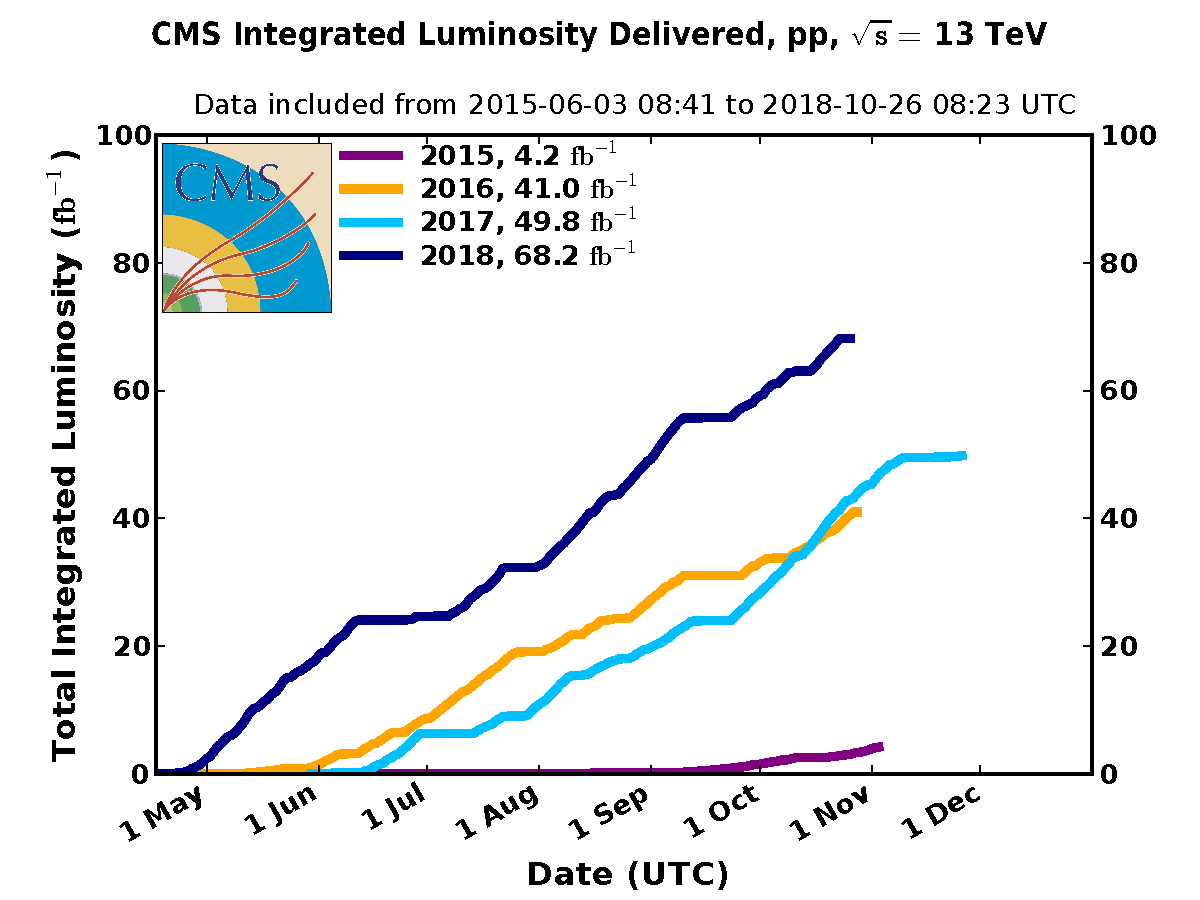
\includegraphics[width=0.5\textwidth]{figures/cms/lumi.pdf}
        \caption{Integrated luminosity of the LHC during proton collisions during Run 2~\cite{lumitwiki}.
	         The results in this thesis use the 2016 dataset.
		 While a total luminosity of 41 \fbinv~ was collected, we only use a subset during which the detector operated optimally.
		 This corresponds to 36 \fbinv~ of data.}
        \label{fig:cms:lumi}
    \end{center}
\end{figure}

\section{The Compact Muon Solenoid}

The Compact Muon Solenoid (CMS)~\cite{cmsjinst} is one of two general purpose LHC detectors, the other being ATLAS~\cite{atlasjinst}.
It is designed to detect and measure stable hadrons, photons, electrons, and muons produced in proton and ion collisions at LHC interaction point 5. 
From these event descriptions, a number of physics processes can be probed, including SM measurements, BSM searches, and the discovery of the Higgs boson. 
In what follows, we will use the $(r,\phi,\eta)$ coordinate system with respect to the $z$ axis:
\begin{itemize}
    \setlength\itemsep{1pt}
    \item $z = $ distance along beam axis, with $z=0$ at the center of the detector
    \item $r = $ distance from the $z$ axis
    \item $\phi = $ azimuthal angle in the plane orthogonal to the $z$ axis
    \item $\eta = $ pseudorapidity $(-\log\nicefrac{\theta}{2}$), with respect to the polar angle $\theta$ 
\end{itemize}
In this coordinate system, we define $x$ and $y$ to lie in the plane perpendicular to $z$, with $x$ pointing from the center of the detector to the center of the LHC.
As with the pseudorapidity, it is convenient to use quantities invariant under $z$-boosts, and so we define the transverse momentum:
\begin{equation}
    \vec{p}_\mathrm{T} = \left(\begin{matrix} p_x \\ p_y \end{matrix}\right)
\end{equation}
We will frequently make use of the magnitude of this vector, $\pt$. 
CMS can detect collision products that are within the fiducial volume of $0 \leq \phi < 2\pi$ and $-5 \leq \eta\leq 5$. 
Several detector subsystems (Figure~\ref{fig:cms:cms}) are used to identify and reconstruct muons, electrons, photons, and charged and neutral hadrons. 

\begin{figure}[]
    \begin{center}
        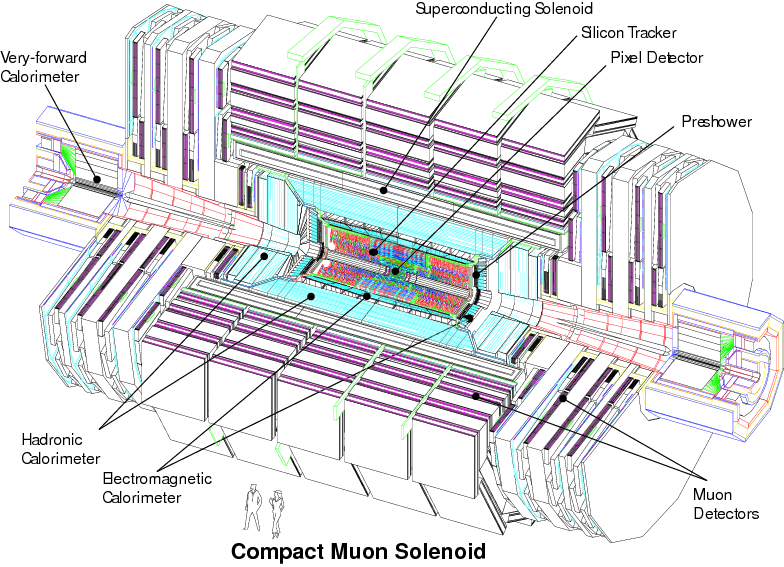
\includegraphics[width=0.65\textwidth]{figures/cms/cms.png}
        \caption{Cut-away view of the CMS detector and its subsystems.
                 Reprinted from Reference~\cite{cmsjinst}.}
        \label{fig:cms:cms}
    \end{center}
\end{figure}

\subsection{Silicon tracker}
\label{sec:cms:tracker}

Starting from the beam pipe, the first of these subsystems is the silicon tracker~\cite{cmstracker}, used to identify charged particles and measure their momenta. 
The tracker consists of silicon detector geometries: pixels (providing 3D position measurement) and strips (2D). 
The arrangement of the pixel and strip layers are shown in Figure~\ref{fig:cms:si}.
A superconducting NbTi solenoid envelopes the tracker, as well as parts of the calorimeters. 
The magnetic field inside the tracker volume has strength 3.8 T and field lines approximately parallel to the beam direction. 

\begin{figure}[]
    \begin{center} 
        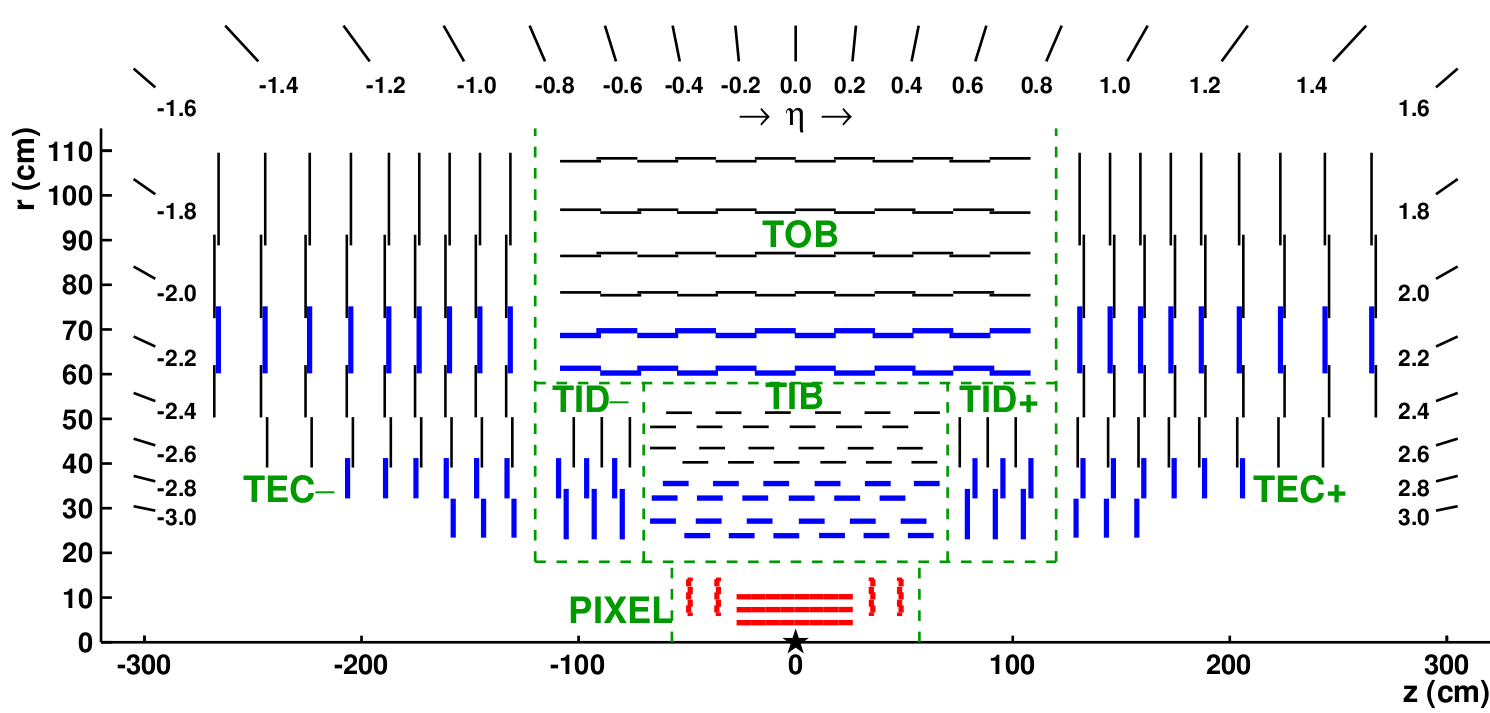
\includegraphics[width=0.7\textwidth]{figures/cms/tracker.png}
        \caption{Diagram of a slice of the CMS tracking system.
                 The pixel layers are shown in bold red lines.
                 Single-strip (double-strip) layers are indicated by thin black (bold blue) lines.
                 The double-strip modules each consist of two back-to-back strips, rotated with respect to each other, that can provide 3D localization of the hits.
                 Reprinted from Reference~\cite{cmstracker}.}
        \label{fig:cms:si}
    \end{center}
\end{figure}


A single silicon pixel has dimensions $285\times100\times150$ $(\mu\mathrm{m})^3$ (in $r\times r\phi\times z$), leading to a position resolution of $\sim10\times30$ $(\mu\mathrm{m})^2$ (in $r\phi\times z$). 
The 66 million pixels are arranged into 7 layers: 3 cylindrical \emph{barrels} (at $r=4.4,~7.3,~10.2$ cm) and $2\times2$ \emph{endcap} annulli (at $z=\pm34.5,~\pm46.5$ cm). 
Outside the pixel layers are the strip layers, consisting of 9.3 million silicon strips arranged into barrels and endcaps.
The resolution in $r\phi$ varies between $10$ and $50$ $\mu$m, depending on the location and pitch of the given strip.
Certain strip layers contain two layers of strips, rotated through a \emph{stereo} angle (100 mrad) with respect to each other.
By matching adjacent hits, the stereo measurement can add a third dimension ($z$ for barrel, $r$ for endcap) to the strip's 2D measurement, with resolution $100$-$500$ $\mu$m.
There are a total of 10 barrel layers ($0.2 < r < 1$ m) and 24 endcap layers ($0.6 < |z| < 2.8$ m). 
Figure~\ref{fig:cms:trackermat} shows that the thickness of the tracker is between 0.4 and 2 electron radiation lengths ($X_0$).

\begin{figure}[]
    \begin{center} 
        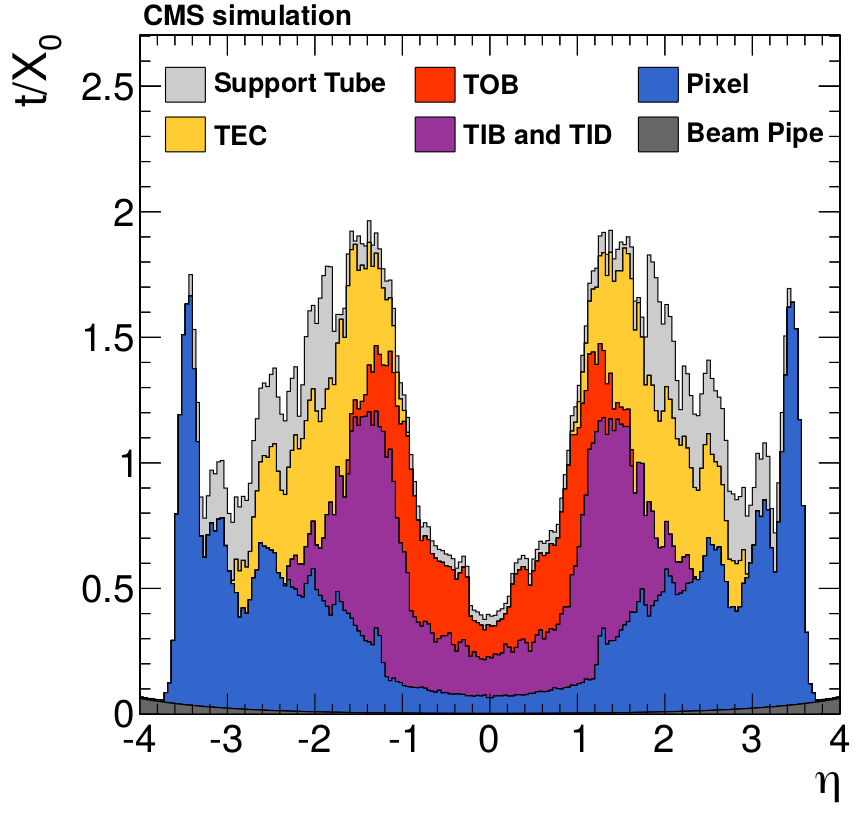
\includegraphics[width=0.5\textwidth]{figures/cms/tracker_material.png}
        \caption{The thickness of the various tracker subsystems and other structures as a function of $\eta$.
				 The $y$-axis is in units of electron radiation length $X_0$.
                 Reprinted from Reference~\cite{cmstracker}.}
        \label{fig:cms:trackermat}
    \end{center}
\end{figure}


Pixels with a signal greater than a tuneable readout threshold (typically around $3000 Q_e$) are read out.
These pixels are then aggregated with adjacent signals to form pixel clusters, which are further subjected to readout thresholds ($\sim 4000 Q_e$).
The exact position of the particle in this layer (known as a \emph{hit}) is inferred by fitting the charge distribution of the pixels in this cluster to pre-determined templates.
A similar method is employed to determine the strip hit positions, with some modifications to account for Lorentz drift of the charges in the silicon detector due to the $B$-field. 
The efficiency of reconstructing hits varies with the detector type, location, and particle momentum, but is generally greater than $99\%$ ($99.5\%$ if defective modules are not considered). 

\subsubsection{Tracking}

Tracks are found using an iterative \emph{inside-out} process, where each iteration has five steps:
\begin{enumerate}
    \item Define seeds using pixel hits, double-strip hits (i.e. hits with 3D information), and an estimate of the beam spot (collision point). At least 3 hits are needed for the seed.
    \item Use a Kalman filter~\cite{kalman2,kalman1} to evolve track seeds through the rest of the tracker and find hits, accounting for the $B$-field, energy loss, and multiple scattering.
    \item Estimate trajectory parameters after finding all hits.
    \item Decide whether to keep found tracks based on quality requirements (e.g. number of missing hits, track $\chi^2$)
    \item Remove hits associated with tracks from hit collection and repeat.
\end{enumerate}
The trajectory parameters referred to in step 3 are the 5 parameters of a helix: $\rho$ (curvature), $\phi_0$ (azimuthal angle), $\lambda$ ($\cot\theta$), $d_0$ (\emph{impact parameter}, minimum $r$ of track), $z_0$ (minimum $|z|$ of track).
The CMS track fit typically has 5-7 iterations, with each successive iteration loosening the seed and track fit requirements to look for more difficult tracks (e.g. missing hits, large $d_0$).
The efficiency and fake rate of this reconstruction, as a function of track \pt, are shown in Figure~\ref{fig:cms:trackeff}.
For muons with $|\eta|<1.5$ and $\pt>1$ GeV, the tracking efficiency is over 98\%, with a combinatorial fake rate of 2-6\%. 

\begin{figure}[]
    \begin{center} 
        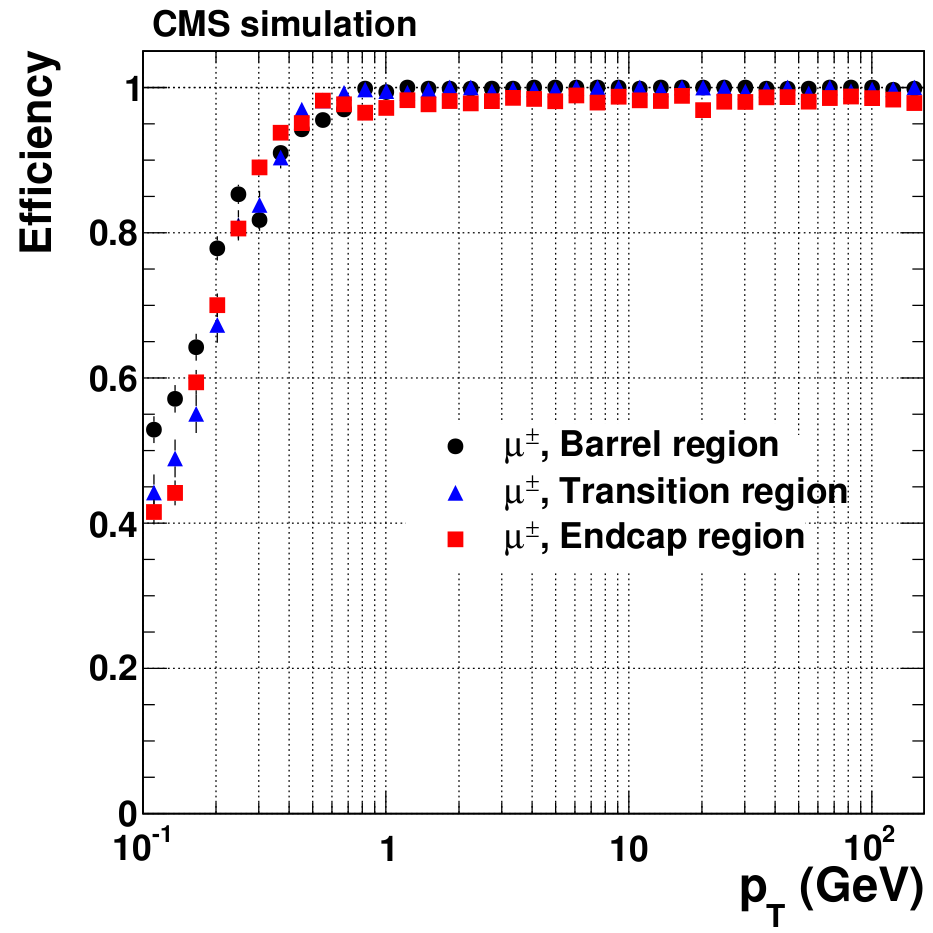
\includegraphics[width=0.36\textwidth]{figures/cms/track_eff.png}
        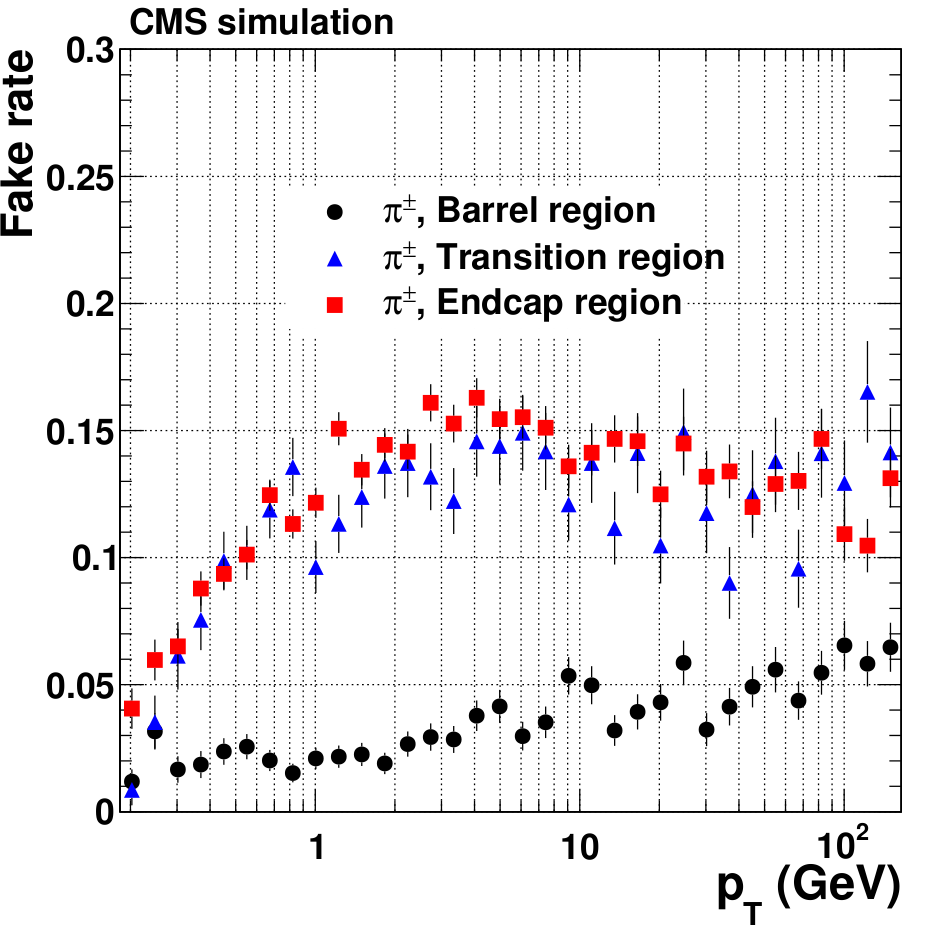
\includegraphics[width=0.36\textwidth]{figures/cms/track_fake.png}
        \caption{Efficiency (fake rate) of the CMS track fit algorithm, evaluated using simulation of muons (charged pions).
                 Reprinted from Reference~\cite{cmstracker}.}
        \label{fig:cms:trackeff}
    \end{center}
\end{figure}

\subsubsection{Vertexing}

The excellent position resolution of the pixel detector is used to accurately measure the position of primary vertices, as well as any secondary vertices from the decays of longer-lived particles with lifetimes $\gtrsim 10^{-13}$ s.
In the former case, tracks are first clustered together on the basis of the likelihood that the tracks in a cluster arise from a single primary vertex.
This is done using a deterministic annealing algorithm~\cite{da}, which has as free parameters the number of clusters and the probability of each track belonging to each cluster.
Having determined the clusters, an adaptive fit algorithm~\cite{adaptivefit} is used to determine the vertex for each cluster.
The free parameters of this fit are the three spatial coordinates of the vertex.
As the LHC collides bunches of $\mathcal{O}(10^{11})$ protons, we expect multiple primary vertices in a single collision, and this is reflected in Figure~\ref{fig:cms:npv}.
The vertex defined to be the hard scattering interaction (known as \emph{the} primary vertex\footnote{This nomenclature is indeed confusing, defining the singular primary vertex to be one of many primary vertices. However, it is standard terminology in CMS publications, so we will continue to use it. In what follows, the distinction will be clear}) is the vertex which maximizes:
\begin{equation}
    \sum_{j\in\text{track jets}} (\pt^j)^2 + (\ptmiss)^2
\end{equation}
where ``track jets`` refer to jets (Section~\ref{sec:cms:jets}) clustered from the vertex's tracks, and \ptmiss~is defined in Section~\ref{sec:cms:met}.
If there are more than 2 charged particle tracks in an event, the efficiency of reconstructing and identifying the correct primary vertex (PV) is greater than $0.995$.
The efficiency does not depend strongly on the total number of reconstructed primary vertices $N_\mathrm{PV}$.

\begin{figure}[]
    \begin{center} 
        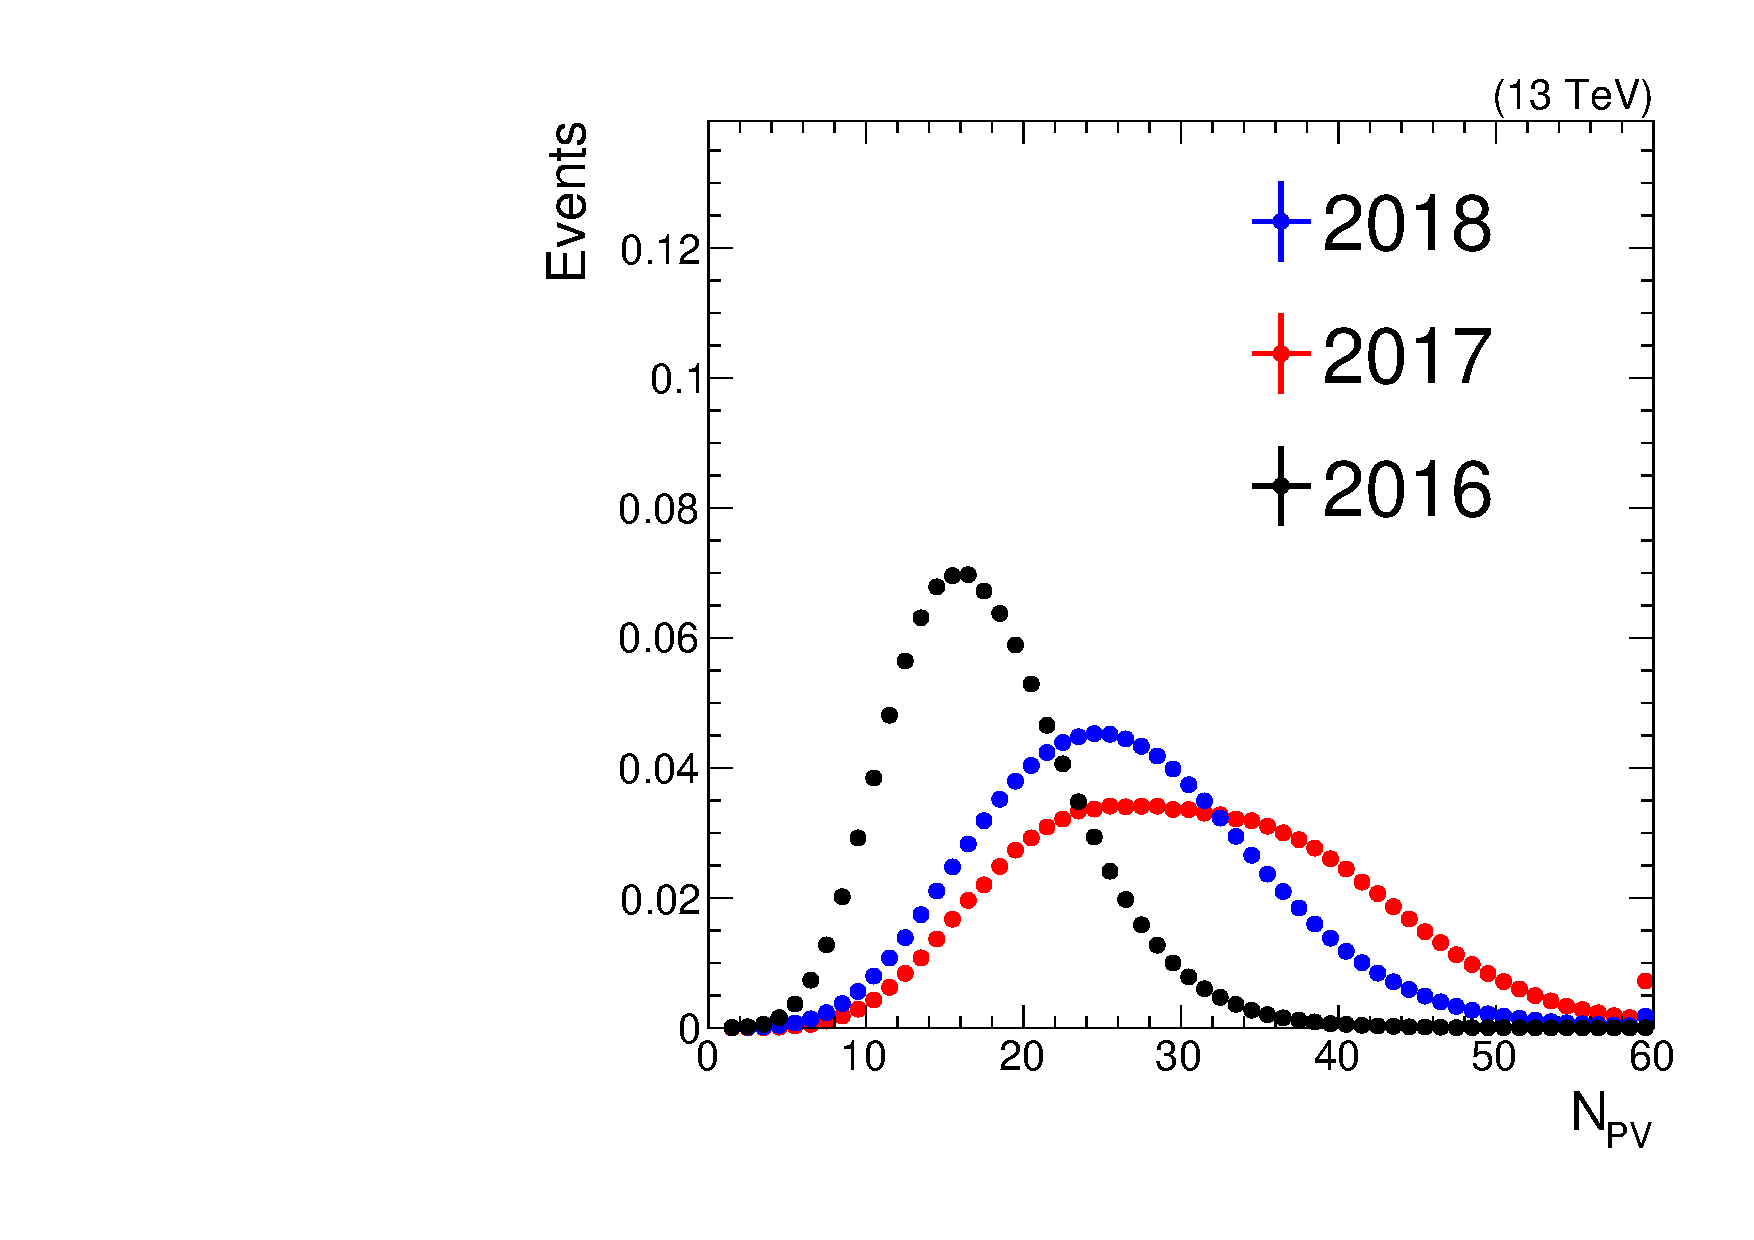
\includegraphics[width=0.6\textwidth]{figures/cms/comparison_npv.pdf}
        \caption{The distribution of the number of reconstructed primary vertices in data recorded by CMS during Run 2 of the LHC.
                 While the results in this thesis only concern 2016 data, we show the evolution of $N_\mathrm{PV}$ as a function of time, as this correlates directly with increased instantaneous luminosity.}
        \label{fig:cms:npv}
    \end{center}
\end{figure}

\subsubsection{Secondary vertexing}

The last reconstruction algorithm concerning the tracker alone is the identification of secondary vertices (SVs), which arise from the decay of longer-lived particles.
The longer-lived particles in the SM are $\tau$ leptons and hadrons containing $b$ and $c$ quarks.
The inclusive vertex fitter (IVF)~\cite{csvv2} reconstructs such secondary vertices by the following steps:
\begin{enumerate}
    \item Select a track as a seed if it satisfies $\sqrt{d_0^2 + d_z^2} > 50~\mu\mathrm{m}$ and $d_0 > 1.2 \delta d_0$.
    \item Choose nearby tracks based on their closest distance to and opening angle with the seed track.
    \item Fit the tracks to a displaced vertex using the adaptive fitter~\cite{adaptivefit}.
    \item Decide which tracks belong to the candidate secondary vertex and which belong to the primary vertex.
    \item Re-fit the secondary vertex position only using the former set of tracks from the previous step.
\end{enumerate}
It is important not only to properly determine the location of the secondary vertex, but also to properly assign tracks.
Observables that are a function of the \emph{tracks} (e.g. vertex mass) will be critical for $b$ jet tagging.

\subsection{Electromagnetic calorimeter}

The CMS electromagnetic calorimeter~\cite{cmsecaljinst} (ECAL) is a homogenous detector with good energy and angular resolution, composed of 76,000 \pbwo~crystals. 
The crystals are arranged in two sections: a cylindrical barrel (EB) covering $|\eta|<1.44$ and two endcap annuli (EE) extending to $|\eta|<3$.
This provides slightly more coverage than the tracking volume.
Each crystal in the EB (EE) has dimensions $2.2\times2.2\times23$ ($2.68\times2.68\times22$) $(\mathrm{cm}^3)$, with the long dimension pointing towards the beam.
This can be compared to a Moli\'ere radius $r_M=2.19$ cm and a radiation length of $X_0=0.89$ cm. 
A cross-sectional area comparable to $r_M\times r_M$ facilitates the differentiation of different electromagnetic (EM) showers arising from electrons and photons.
The depth of the crystal (in units of $X_0$) drives the excellent energy resolution, which is determined using an electron beam:
\begin{equation}
    \frac{\sigma_E}{E} = \frac{2.8\%}{\sqrt{E/\mathrm{GeV}}} \oplus \frac{12\%}{E/\mathrm{GeV}} \oplus 0.3\%
\end{equation}
Scintillation photons from the \pbwo~crystals are collected by avalanche photodiodes (APDs) in the EB and vacuum phototriodes (VPTs) in the EE, which provide amplification factors of 50 and 10, respectively. 

At high momenta, the two photons from a $\pi^0$ decay may merge into a single ECAL crystal. 
This primarily occurs at high $|\eta|$ due to the $z$-boost of the intitial state.
To differentiate one- and two-photon deposits, a \emph{preshower} detector sits in front of the EE ($1.6 < |\eta|<2.5$).
The preshower detector consists of a lead absorber and silicon strips.
A photon (or photon pair) initiates a shower in the lead.
The shower can be resolved in the silicon strips, which have resolution $\mathcal{O}(1\mathrm{-}10)$ mm.

The physical placement of all three ECAL components is shown in Figure~\ref{fig:cms:ecal}.

\begin{figure}[]
    \begin{center} 
        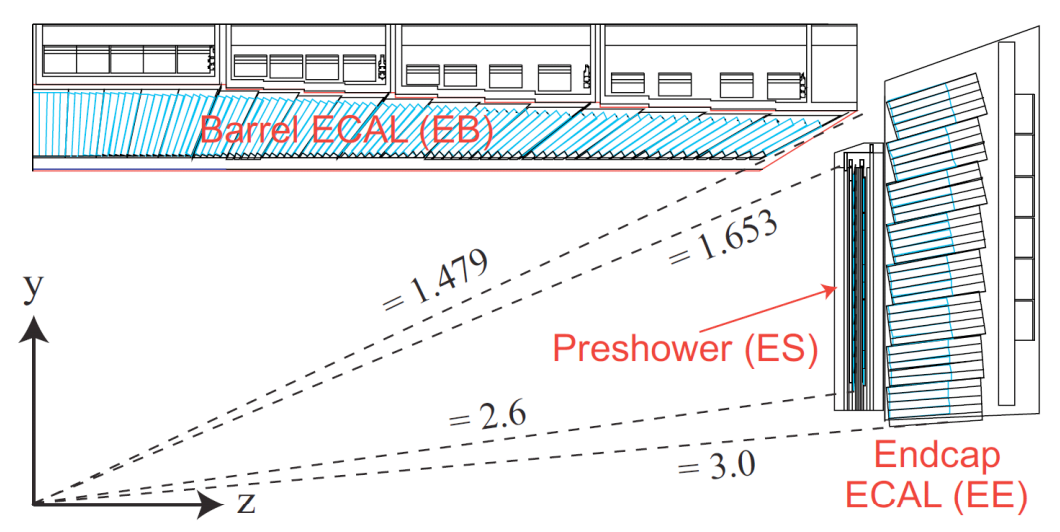
\includegraphics[width=0.7\textwidth]{figures/cms/ecal.png}
        \caption{One quadrant of the CMS ECAL (symmetric with rotation around $z$ and reflection across $z=0$).
                 The dashed lines indicate values of $\eta$.
                 Reprinted from Reference~\cite{cmsecaljinst}.}
        \label{fig:cms:ecal}
    \end{center}
\end{figure}

Due to the bending of a charged particle's trajectory in the solenoidal $B$-field and interactions with the tracker material, bremsstrahlung photons will be emitted at similar values of $\eta$, but spread along $\phi$.
A \emph{supercluster} (SC) is defined by clustering nearby ECAL energy depositions, allowing for a wider spread in $\phi$ than in $\eta$ (Figure~\ref{fig:cms:sc}).
The particle's EM energy is defined to be the weighted sum of the energies of all crystals in the SC, where the coefficients account for crystal-specific calibration effects~\cite{cmsecalreco}.
For an electron or photon, the EM energy is typically the energy of the particle, whereas for other particles (charged hadrons and muons), it is only a fraction of the total energy.

\begin{figure}[]
    \begin{center} 
        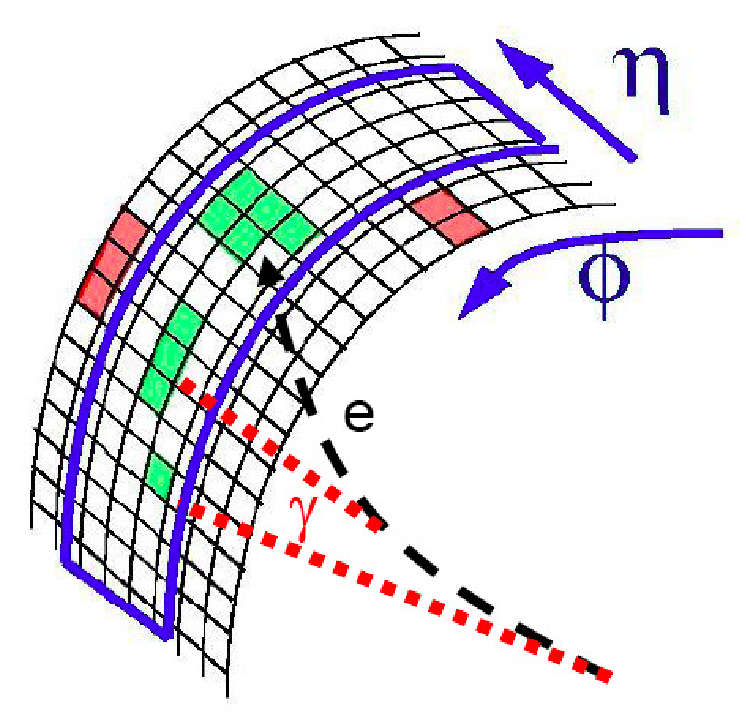
\includegraphics[width=0.3\textwidth]{figures/cms/sc.png}
        \caption{The combination of multiple ECAL crystals into a single supercluster, intended to capture energy depositions from bremsstrahlung photons.
                  Reprinted from Reference~\cite{cmsecalrev}.}
        \label{fig:cms:sc}
    \end{center}
\end{figure}

\subsection{Hadronic calorimeter}

The hadronic calorimeter (HCAL)~\cite{cmshcaltdr,cmspf,cmshcalperf} is used to identify and measure the energy of hadrons.
It consists of 4 calorimeters: barrel (abbreviated HB, covering $|\eta|<1.4$), endcap (HE, $1.3<|\eta|<3$), forward (HF, $3\lesssim|\eta|<5$), and outer (HO, $|\eta|<1.3$).
Their arrangement is shown in Figure~\ref{fig:cms:hcal}.

\begin{figure}[]
\begin{center}
    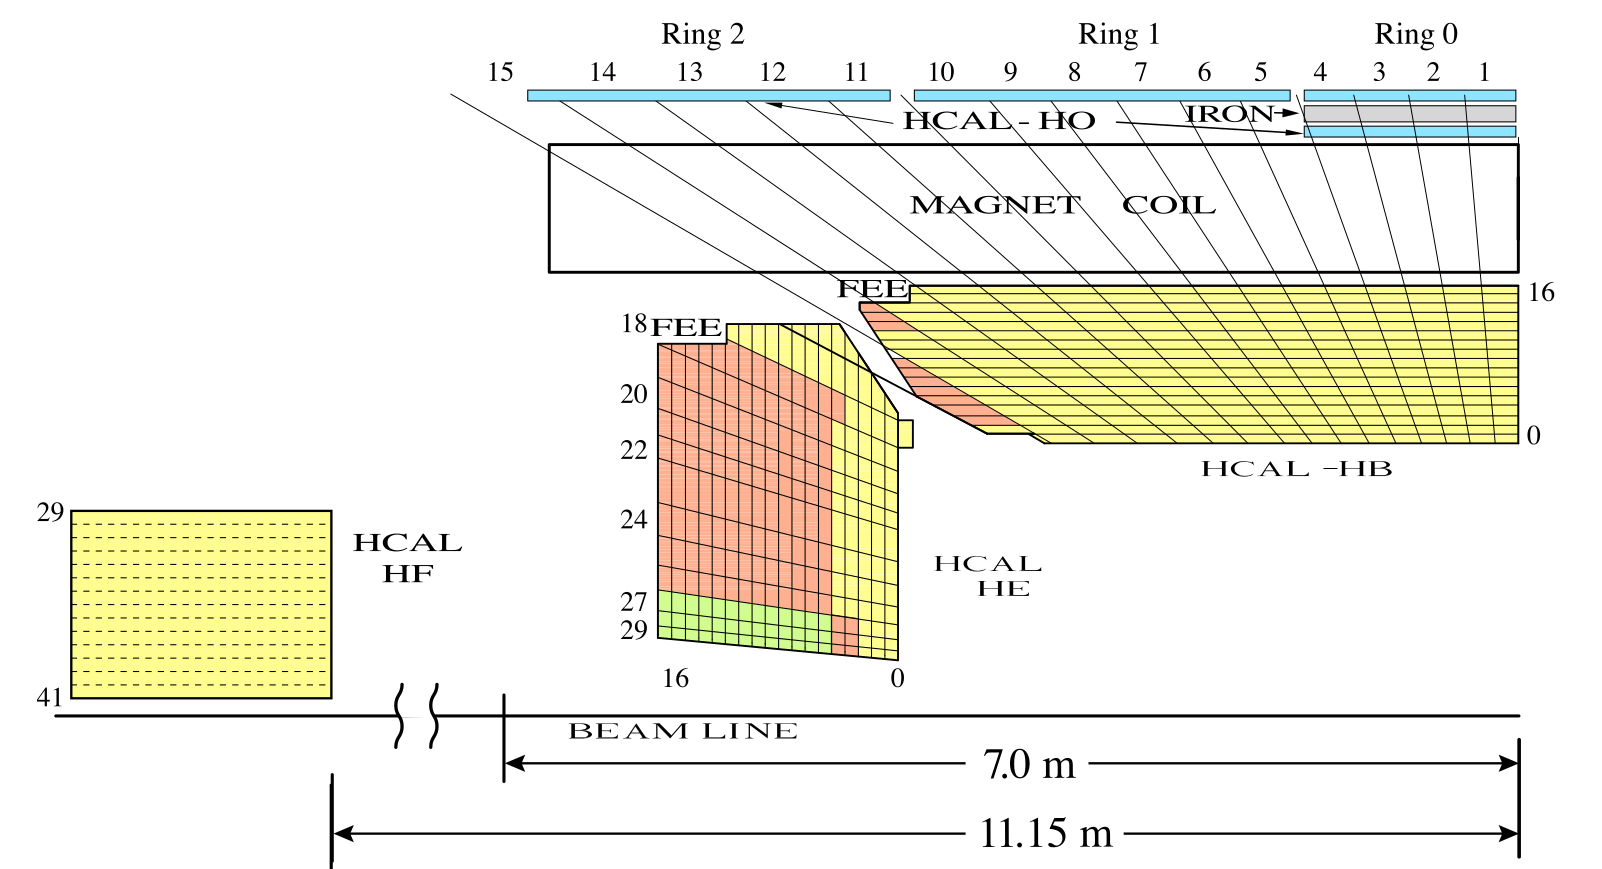
\includegraphics[width=0.7\textwidth]{figures/cms/hcal.png}
    \caption{One quadrant of the CMS HCAL (symmetric with rotation around $z$ and reflection across $z=0$).
             Note that the slight overlap of the detectors in $\eta$ ensures the hermeticity of the detector.
             Reprinted from Reference~\cite{cmshcalperf}.}
    \label{fig:cms:hcal}.
\end{center}
\end{figure}

The HB and HE are both composed of alternating absorber and plastic scintillator layers.
The absorber is a non-magnetic brass alloy with an interaction length $\lambda_I=1.5$ cm.
Absorber layers range in thickness from 40 to 75 mm in the HB and HE, providing a total of 5.8-10.6~$\lambda_I$ of material, depending on the $\eta$ of the particle.
These dimensions are limited by the constraint that the HB and HE be inside the solenoid. 
To augment the number of interaction lengths, additional layers of plastic scintillator are located outside of the solenoid.
These comprise the HO, which use the magnet as an absorber, providing an additional $\sim 1.1~\lambda_I$.
The light from the scintillator tiles is read out by hybrid photodiodes (HPDs) in the HB and HE and by silicon photomultipliers (SiPMs) in the HO. 

Beyond the HE, at 11 m from the interaction point, is the HF.
The HF is also a sampling calorimeter, made of steel absorbers instrumented with quartz fibers.
Charged particles from the nuclear shower in the steel emit Cerenkov radiation as they traverse the quartz fibers, which transports the light to photomultipler tubes (PMTs).
The HF uses more radiation-hard materials than the rest of the HCAL because this $\eta$ range is subject to significantly more radiation from collisions than the central part of the detector (Figure~\ref{fig:cms:flux}). 

\begin{figure}[]
    \begin{center}
        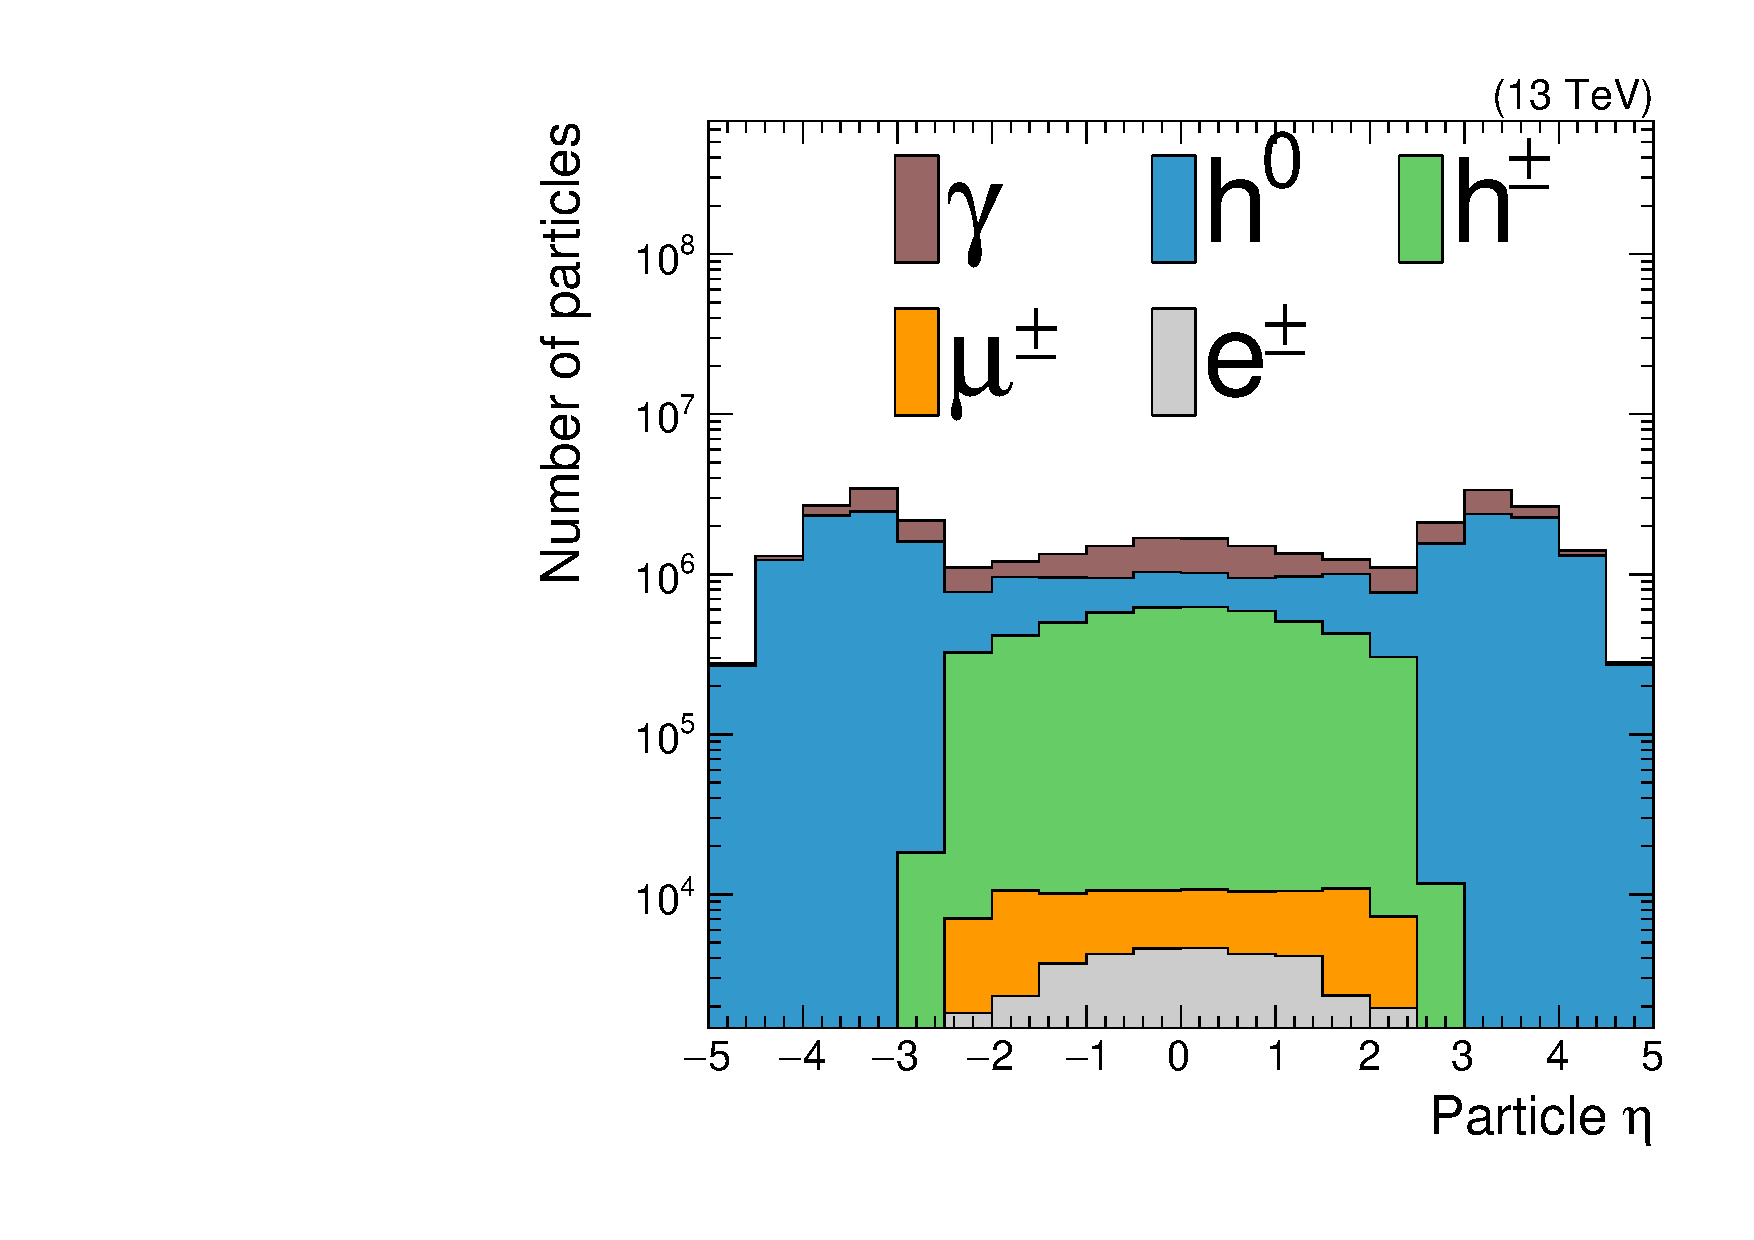
\includegraphics[width=0.6\textwidth]{figures/cms/flux.pdf}
        \caption{Flux of various particle types as a function of $\eta$ in the detector.
             The symbol $h$ refers to any type of hadron.
             Note that $h^0$ ($\gamma)$ is used to refer to any neutral or charged hadron (photon or electron) in the forward region, where the tracker and ECAL do not have coverage.}
        \label{fig:cms:flux}
    \end{center}
\end{figure}

Each HCAL subsystem is read out in \emph{towers}.
A tower corresponds to a small segment in $\eta$ and $\phi$ and traverses the perpendicular dimension.
The direction of a particle is determined from the tower location.
For $|\eta|<1.74$, the segmentation is $\eta\times\phi = 0.087\times0.087$.
Beyond this, the towers vary in size from $0.09\times0.175$  to $0.35\times0.175$.

The energy resolution of the HCAL must be considered in conjunction with the ECAL, as energy is deposited in both detectors.
This is calibrated using test beams of various charged particles.
For the HB and HE, the combined ECAL+HCAL resolution is:
\begin{equation}
    \frac{\sigma_E}{E} = \frac{0.847}{\sqrt{E/\mathrm{GeV}}} \oplus 0.074
\end{equation}
The region instrumented by the HF does not have ECAL coverage, and so the resolution for the HF alone is:
\begin{equation}
    \frac{\sigma_E}{E} = \frac{1.98}{\sqrt{E/\mathrm{GeV}}} \oplus 0.09
\end{equation}

\subsection{Muon chambers}

The muon detectors are gas ionization chambers and are the outermost component of CMS~\cite{cmsmuon}. 
The chambers are interleaved with the steel return yoke of the CMS magnet, ensuring a $B$-field which runs anti-parallel to the field inside the solenoid.
This results in the characteristic $S$-shape of muon trajectories, as the bending changes direction across the solenoid. 
3 types of ionization detectors are used: drift tubes (DTs; barrel), cathode strip chambers (CSCs; endcaps), and resistive plate chambers (RPCs; barrel and endcaps).
The physical placement of the detectors is shown in Figure~\ref{fig:cms:muondet}.

\begin{figure}[]
    \begin{center}
        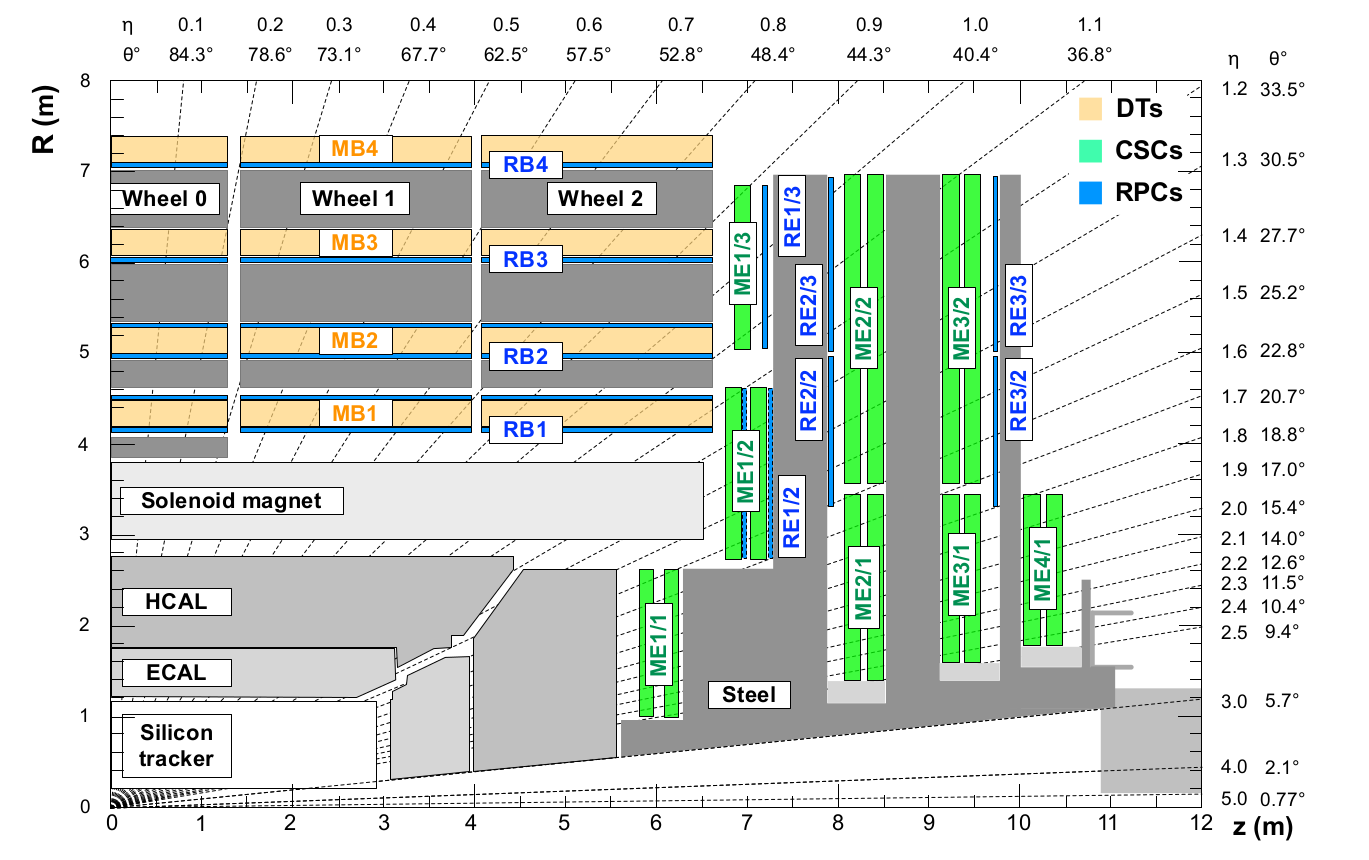
\includegraphics[width=0.7\textwidth]{figures/cms/muon.png}
        \caption{One quadrant of the CMS muon detection system, with the DTs (MBs), CSCs (MEs), and RPCs (RBs/REs) labeled. 
                 Reprinted from Reference~\cite{cmsmuon}.}
        \label{fig:cms:muondet}
    \end{center}
\end{figure}

The DT cells are filled with a 85:15 mix of argon and carbon dioxide, with a gold/steel anode wire held at a voltage of $3600$ V.
The cell is a rectangular prism, with transverse dimensions of $42\times13~\mathrm{mm}^2$ and a longitudinal dimension ranging from $1.9$ to $4.1$ m.
The dimensions and the drift speed of $55~\mu\mathrm{m/s}$ result in a maximum response (drift) time of $400$ ns.
The DTs are organized into cylindrical \emph{stations} (MB).
With the exception of the outermost barrel station (MB4), each MB consists of 3 \emph{superlayers} (SLs).
Each SL has 4 parallel drift cells, and so measure position in a particular plane.
Of the 3 SLs, two measure $r$-$\phi$ position and one measures $r$-$z$ position. 
MB4 does not have an $r$-$z$ SL.

The endcap is instrumented with CSCs as these have a faster response time and better spatial resolution than DTs.
This is needed in the forward region, where both the muon and background fluxes are higher.
While the CSC dimensions vary depending on the position of the chamber, each is instrumented with 80 cathode strips, held at voltages (relative to the anode) of 2.9-3.6 kV.
The CSC wires have a separation of 2.5-3.16 mm, which governs the position resolution.
A 50:40:/10 mix of $\mathrm{CO}_2/\mathrm{Ar}/\mathrm{CF}_4$ is used to fill the chambers.

RPCs are interspersed among the DTs and CSCs in both the barrel and endcap. 
These serve as a very fast muon detector ($\sim 1$ ns) for the online trigger system. 
The spatial resolution of the RPC hits is worse than the DTs and CSCs.

The hit position resolution of the DTs is 78-120 $\mu$m (140-390 $\mu$m) in $r$-$\phi$ ($r$-$z$).
For CSCs, the resolution varies from 40 to 152 $\mu$m.
The efficiency of individual reconstructed hits (\emph{rechits}) is over 95\%.

\subsection{Online trigger system}

Figure~\ref{fig:cms:xsecs} shows various cross sections of $pp$ collisions as a function of $\sqrt{s}$.
While it is clear that interesting SM processes increase as a function of $\sqrt{s}$, their cross sections are still several orders of magnitude below the inclusive cross section $\sigma_\mathrm{tot}\sim 10^8$ nb.
To produce an appreciable number of rare events, the LHC has bunch crossings every 25 ns (40 MHz).
However, it is not possible to read out the entire detector at this rate, much less reconstruct the data and store it.
CMS uses a two-stage trigger system~\cite{cmstrig} to refine the events to keep for permanent storage and analysis.
First, a Level 1 (L1) hardware-based trigger selects interesting events at a rate of 100 kHz.
The L1 makes these decisions using incomplete detector information, in order to reduce the read-out and computation time.
Selected events are then fed to the high level trigger (HLT) to partially reconstruct the events on a CPU farm.
The HLT uses the full granularity of the detector.
The final selected data rate from the HLT is 400 Hz.

\begin{figure}[]
\begin{center}
    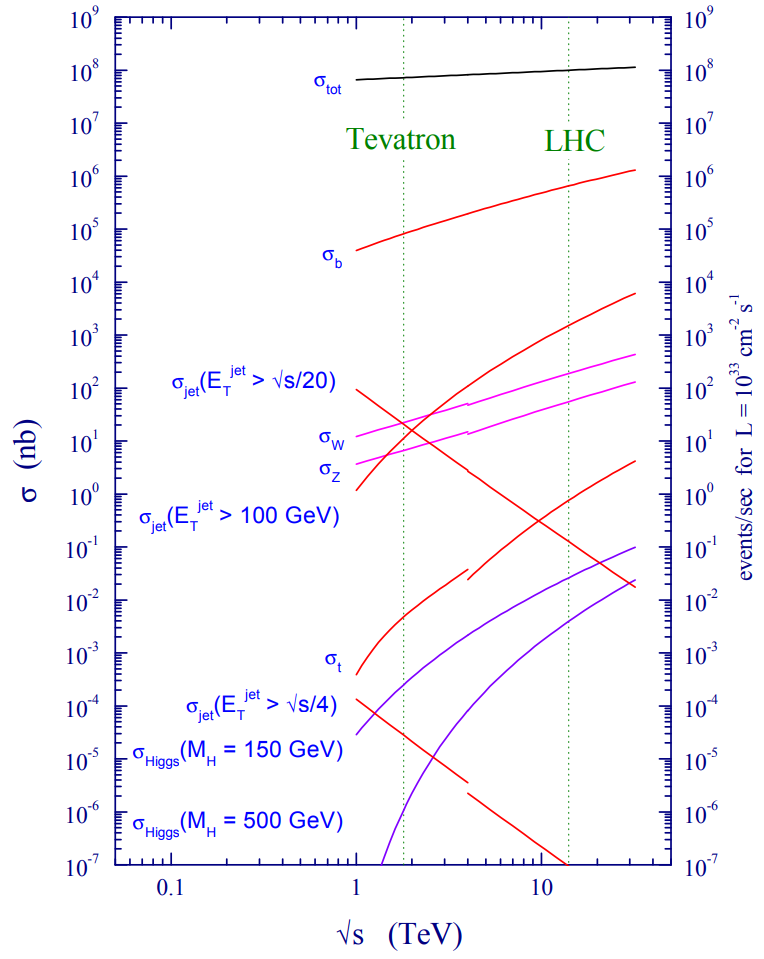
\includegraphics[width=0.7\textwidth]{figures/cms/xsec.png}
    \caption{Various cross sections of interesting SM processes compared to the inclusive cross section of $pp$ collisions, at various values of $\sqrt{s}$.
                Reprinted from Reference~\cite{lhcxsec}.}
    \label{fig:cms:xsecs}
\end{center}
\end{figure}

\subsubsection{Level 1}

The L1 trigger makes decisions within 4 $\mu$s of collisions using field programmable gate arrays (FPGAs) and application specific integrated circuits (ASICs), which offer significant speed advantages as compared to CPUs for certain tasks.
Individual detector systems (ECAL, HCAL, muon detectors) feed simple reconstructed objects (\emph{trigger primitives} (TPs)) to a series of regional trigger decisions.
Quality selections are placed on calorimeter towers, and they are aggregated into clusters of energy deposits.
A simple segment-finding and tracking algorithm is run on hits in the muon chambers to produce muon tracks.
Note that the inner tracker is not included in the L1 decision: at the time of the construction of the CMS detector, the detector readout and reconstruction algorithms were not fast enough for the L1's requirements.\footnote{It should be noted that implementing tracking for hardware triggers is a significant goal for the community in the next few years.}
Regional trigger decisions are sent to the global trigger (GT), which correlates the TPs it recieves.
Some GT trigger decisions are localized, such as requiring a high-energy ECAL deposit (e.g. $e,\gamma$).
Others require computing event-wide observables, such as a large momentum imbalance (e.g. neutrinos, DM).
The GT also computes simple jets.
If the GT decides to select the event, the detector is read out and forwarded to the data acquisition system (DAQ).
Figure~\ref{fig:cms:l1} shows a schematic description of this process.

\begin{figure}[]
\begin{center}
    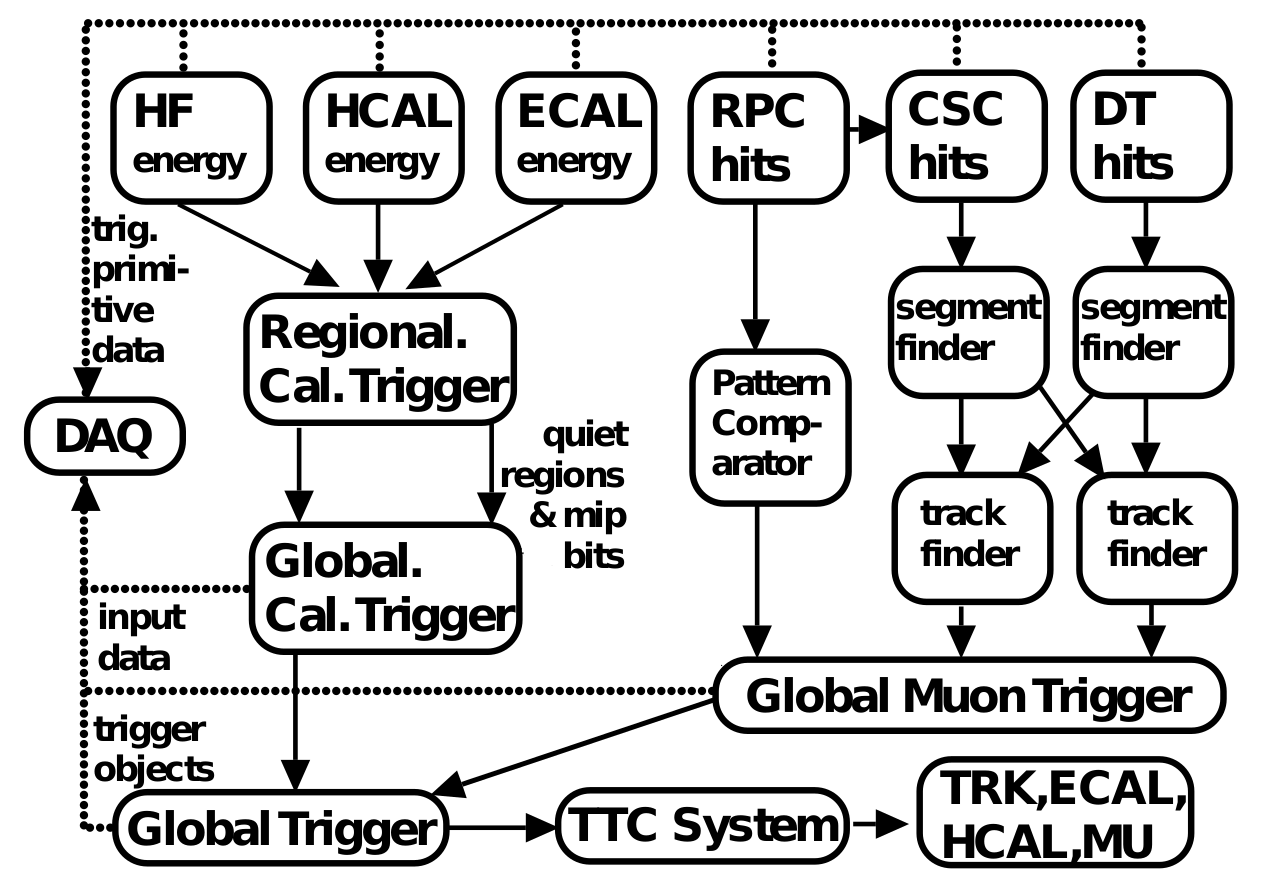
\includegraphics[width=0.65\textwidth]{figures/cms/l1.png}
    \caption{Schematic diagram of the CMS L1 trigger system.
             In addition to the region and global trigger decisions, the flow of data also includes the trigger, timing, and control system (TTC).
             Reprinted from Reference~\cite{cmstrig}.}
    \label{fig:cms:l1}
\end{center}
\end{figure}

\subsubsection{High level trigger}

The full detector readout is picked up by the HLT.
The HLT computing farm consists of 20k CPU cores (this number has grown from 13k in 2012 and continues to grow).
Unlike the L1, the HLT has access to the entire event information.
Therefore, a full reconstruction of the event is performed, using algorithms similar to those used in offline reconstruction.
To be selected by the HLT, an event must pass an HLT \emph{path}.
A path consists of a series of filters, each making simple decisions that can be chained into complex decisions.
For example, three filters may be: (1) two forward jets, (2) large momentum imbalance, and (3) an electron and a muon.
These filters could be chained into two separate paths, targeting vector boson fusion production of the Higgs, where the Higgs decays to DM (1\&2) or two taus (1\&3).
Simple decisions (calorimeter and muons) are computed before complex decisions (tracking).
Events that are selected by the HLT are passed on to the Tier 0 computing farm for full offline reconstruction, and then onwards to disk and tape resources for analysis and storage, respectively.



\section{Particle reconstruction and identification}

\subsection{Particle flow algorithm}

The excellent angular granularity of the CMS detector and the momentum resolution of the tracker are leveraged by the \emph{particle flow}~\cite{cmspf} algorithm, which correlates information from all detector subsystems to build a global description of each event.
Particle flow (PF) algorithms date back to ALEPH~\cite{alephpf}.

The key feature of the PF algorithm is to \emph{link} multiple detector signals together into a single PF candidate.
This linkage combines inner tracks, ECAL clusters, HCAL clusters, and muon tracks based on their proximity in the $(\eta,\phi)$ plane.
Inner track helices are extended into the calorimeters, searching for clusters compatible with the trajectory.
Similarly, clusters from the ECAL, the ECAL preshower, and the HCAL can be linked without a track present. 
The remainder of this section is organized according to \emph{blocks} in the PF algorithm.
At the end of each block, any detector signature (track, calorimeter cell) which has been assigned to a PF candidate in that block is removed from the set of objects passed to the next block.
For example, tracks associated with muons will not be considered when reconstructing charged hadrons. 

\subsection{Muons}
\label{sec:cms:muons}

The first block of the PF algorithm links inner tracks and muon chamber hits to identify muons.
While \emph{standalone} muons can rely solely on muon chamber hits, we also consider muons that use the inner tracker.
To construct outside-in \emph{global muons}, standalone muon tracks are first reconstructed using a Kalman filter fit using muon chamber rechits~\cite{cmstdr1,cmsmuon}.
These standalone tracks are extrapolated inwards to the inner tracker, accounting for effects from the magnetic field and the  material between the tracker and the muon chambers.
A second Kalman filter fit is run to combine the inner track with the standalone track to form a global muon.
To reject backgrounds, requirements are placed on the $\nicefrac{\chi^2}{N_\mathrm{dof}}$ (poorly fit tracks, charged hadrons) and $d_0,d_z$ (muons from hadron decays and cosmic rays).
The total efficiency of global muon reconstruction is 99\%.
\emph{Tracker} muons are reconstructed from the inside-out, extrapolating inner tracks to the muon chambers and re-fitting with muon rechits.
Figure~\ref{fig:cms:muonpt} compares the momentum resolution of muons reconstructed using the different algorithms.  
The PF selection consumes all three types of reconstructed muons: global, tracker, and standalone.
In this thesis, we will only use global muons.

\begin{figure}[]
\begin{center}
    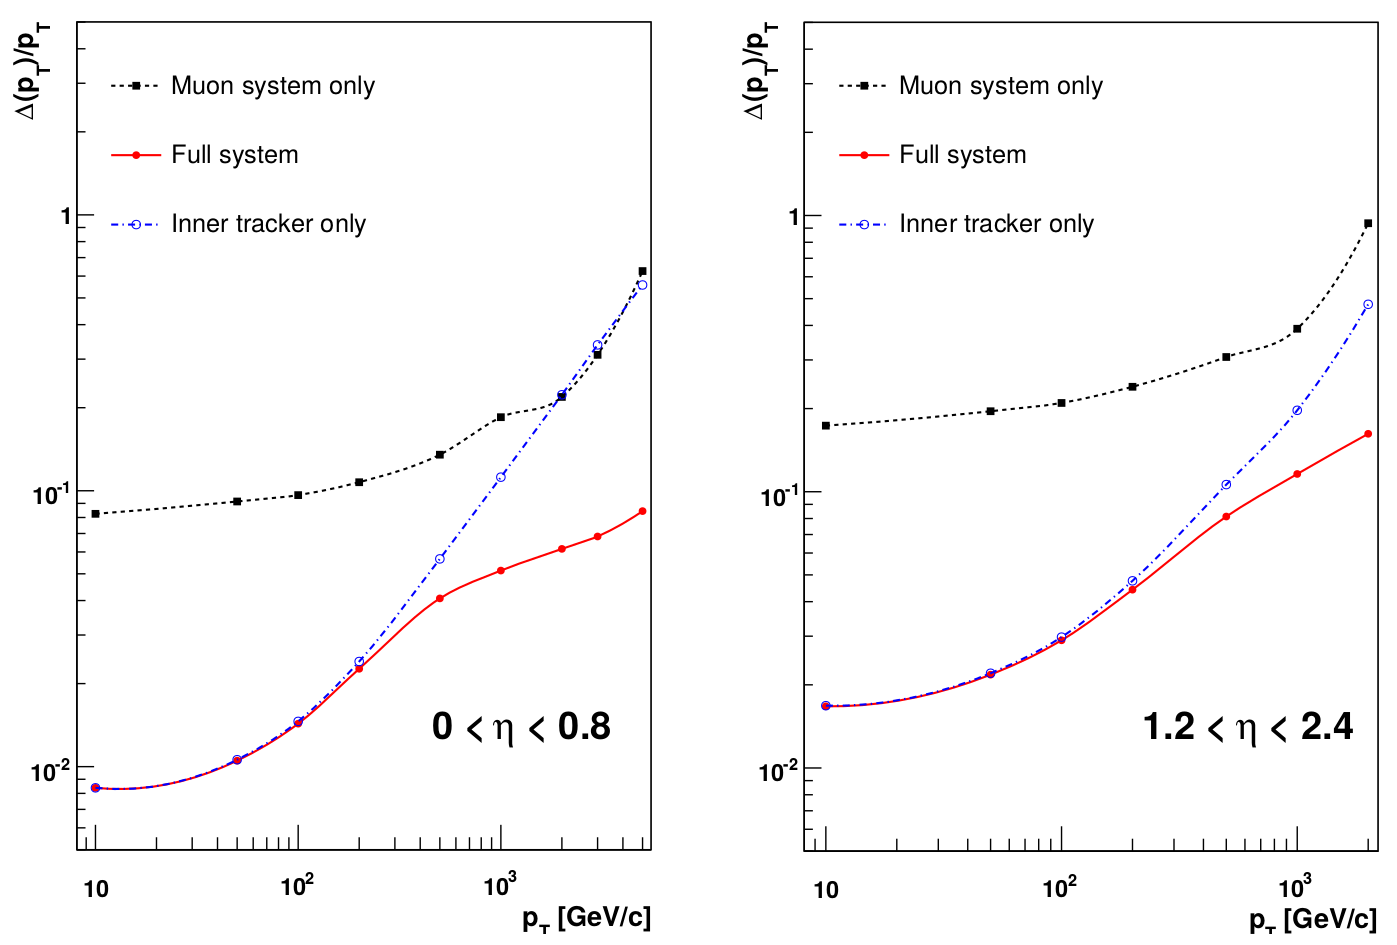
\includegraphics[width=0.6\textwidth]{figures/cms/muonpt.png}
    \caption{Resolution of muon $\pt$, compared between the different reconstruction algorithms. 
             The salient feature is that the muon systems become important to the momentum measurement at approximately 200 GeV.
             Reprinted from Reference~\cite{cmsmuon}.}
    \label{fig:cms:muonpt}
\end{center}
\end{figure}

The PF selection is intentionally non-restrictive, so as to minimize the rate of not identifying a real muon.
To reduce the rate of mis-identified charged hadrons, we define two muon identification (ID) criteria that are slightly stronger than the PF selection. 
The first is a loose ID, which is used to veto muons when defining muon-free data samples.
A loose muon is required to be either a global or tracker muon and have PF isolation less than $0.25$.
PF isolation is defined as:
\begin{equation}
    \left(\sum_{i \in \text{PV charged had.}} \pt^{(i)} +
    \max\left\{0,~\sum_{i\in\text{neut. had.}} \pt^{(i)} + \sum_{j\in\gamma} \pt^{(j)} - 
            \frac{1}{2} \sum_{k\in\text{PU charged had.}}\pt^{(k)}\right\} \right)
    \big/ \pt^{(\mu)}
\end{equation}
where the sums are over PF candidates within $\Delta R < 0.4$ of the muon.
PV and PU refer to the primary vertex and pileup vertices, respectively.
The tight muon ID requires a global muon, PF isolation less than $0.15$, and has selections on the criteria in Table~\ref{tab:cms:muon}.

\begin{table}
    \begin{center}
        \caption{Observables used in identifying muons and rejecting backgrounds}
        \label{tab:cms:muon}
        \begin{tabular}{c|p{0.65\textwidth}}
            Observable & Notes \\ 
            \hline
            \hline
            \pt & Backgrounds grow at low \pt. \\ \hline
            $\chi^2/N_\mathrm{dof}$ & Ensure a good track fit. \\ \hline
            $N_\mathrm{hit}^\mathrm{muon}$ & At least one hit in the muon chamber in the global fit. \\ \hline
            $N_\mathrm{stations}$ & At least two muon chamber stations contain segments of the track. \\ \hline
            $d_0$ & Track impact parameter, remove cosmic rays and hadron decays. \\ \hline
            $d_z$ & Track impact parameter, as above but also for pileup. \\ \hline
            $N_\mathrm{hit}^\mathrm{pixel}$ & At least one pixel hit. \\ \hline
            $N_\mathrm{hit}^\mathrm{tracker}$ & At least 5 hits in the tracker. \\ 
        \end{tabular}
    \end{center}
\end{table}

To account for differences between data and simulation in the performance of the muon IDs, corrections (known as scale factors) are derived:
\begin{equation}
    \SF = \frac{\epsilon_\mathrm{Data}}{\epsilon_\mathrm{MC}}
\end{equation}
where $\epsilon$ refers to the fraction of muons that are correctly identified by the ID criteria.
While $\epsilon_\mathrm{MC}$ is computed directly from MC truth information, $\epsilon_\mathrm{Data}$ is extracted from data using the \emph{tag-and-probe} method~\cite{cmstnp}.
The standard approach starts with $Z\rightarrow\mu\mu$ candidate events with exactly two PF muons.
One muon (the \emph{tag}) is selected using some stringent ID criteria.
Then, the events are categorized by whether the second PF muon candidate (the \emph{probe})  in the event also passes the ID criteria with efficiency.
The number of $Z\rightarrow\mu\mu$ events in each category is measured by fitting the $m_{\mu\mu}$ distribution, which strongly distinguishes between the falling charged hadron background and the $Z$ peak.
The desired ID efficiency is then:
\begin{equation}
	\epsilon_\mathrm{Data} = \frac{N_\mathrm{pass}^{Z}}{N_\mathrm{pass}^Z + N_\mathrm{fail}^Z}
\end{equation}
Note that the efficiency of the tag criteria does not affect $\epsilon_\mathrm{Data}$ as the two muons are statistically independent.
The tag definition is chosen to balance the statistical power and the purity of the sample.

\subsection{Electrons and photons}

Both electrons and photons are seeded using ECAL SCs, with electrons also being associated with an isolated track.
Due to the significant material budget of the silicon tracker, electrons will lose a significant amount of energy through bremsstrahlung.
Although this energy is partially recovered through the supercluster algorithm, the standard Kalman filter tracking fit does not properly account for the non-Gaussian hit uncertainties induced by bremsstrahlung.
Therefore, a modified algorithm based on a Gaussian Sum Filter (GSF)~\cite{cmstracker,gsf} is used to fit the track.
Hits in the pixel and strip endcap layers consistent with the ECAL SC are used to seed the GSF fit.
GSF differs from a Kalman filter by modeling the uncertainties as a Gaussian mixture model instead of a single Gaussian.
The primary backgrounds for electron identification are (1) the overlap of a charged hadron with a neutral hadron or photon and (2) a photon which converts into a $e^-/e^+$ pair in the tracker.
Table~\ref{tab:cms:el} lists the observables used to reject these backgrounds; two cut-based IDs are defined.
The \emph{loose} ID selects electrons with $\sim90\%$ signal efficiency and $\sim0.5\%$ background acceptance (strongly dependent on the electron phase space); it is used to \emph{veto} electrons. 
The \emph{tight} ID selects electrons with $\sim70\%$ signal efficiency and $\sim0.1\%$ background acceptance; it is used to \emph{select} electron-pure samples. 

\begin{table}
    \begin{center}
        \caption{Observables used in identifying electrons and rejecting hadron and photon backgrounds}
        \label{tab:cms:el}
        \begin{tabular}{c|p{0.65\textwidth}}
            Observable & Notes \\ 
            \hline
            \hline
            \pt & Backgrounds grow at low \pt~and brem.~photons can make low-\pt~tracking difficult. \\ \hline
            $\sigma_{i\eta i\eta}$  & Energy-weighted width of cell $\eta$ in SC. Small for electrons. \\ \hline
            $|\Delta\eta(\mathrm{track,SC})|$  & $\Delta\eta$ between SC seed crystal and GSF track at PV. Small for electrons.  \\ \hline
            $|\Delta\phi(\mathrm{track,SC})|$  & $\Delta\phi$, as above.\\ \hline
            $E_\mathrm{H}/E_\mathrm{EM}$  & Ratio of HCAL and ECAL energies. Large for hadrons. \\ \hline
            PF isolation & Sum of energies of other PF candiates near electron. Large for particles in jets. \\ \hline
            $|\nicefrac{1}{E}-\nicefrac{1}{p}|$ & Checks if ECAL and tracker agree ($m_e\sim0$) \\ \hline
            $N_\mathrm{hit}^\mathrm{miss}$ & Conversions or bad tracks will have multiple missing hits in the inner tracker.\\ \hline
            Conversion veto & Check for a pair of tracks originating at a displaced vertex.\\ 
        \end{tabular}
    \end{center}
\end{table}

Photons are defined as ECAL SCs without matched tracks. 
Table~\ref{tab:cms:pho} describes the selection variables used to define the loose veto ID ($\epsilon_\mathrm{sig}\approx90\%$, $\epsilon_\mathrm{bkg}\approx17\%$) and the tight selection ID ($\epsilon_\mathrm{sig}\approx82\%$, $\epsilon_\mathrm{bkg}\approx12\%$).
The direction and energy of a photon are defined by the ECAL SC position and energy, respectively.

\begin{table}
    \begin{center}
        \caption{Observables used in identifying photons and rejecting hadron backgrounds}
        \label{tab:cms:pho}
        \begin{tabular}{c|p{0.65\textwidth}}
            Observable & Notes \\ 
            \hline
            \hline
            \pt & Backgrounds grow at low \pt. \\ \hline
            $\eta$ & EB resolution is better than EE; less hadron background. \\ \hline
            $\sigma_{i\eta i\eta}$  & Defined in Table~\ref{tab:cms:el}. \\ \hline
            $E_\mathrm{H}/E_\mathrm{EM}$  & Defined in Table~\ref{tab:cms:el}. \\ \hline
            PF isolations & Defined in Table~\ref{tab:cms:el}. For photons, separate isolation criteria are placed on each PF type (photon, charged hadron, neutral hadron). \\ 
        \end{tabular}
    \end{center}
\end{table}

To calibrate ECAL SCs, we define the $R_9 = E_{3\times3}/E_\mathrm{SC}$. 
$E_{3\times3}$ is the sum of the energies of the crystals in a $3\times3$ square centered on the most energetic crystal in the SC. 
Much like $\sigma_{i\eta i\eta}$, it is sensitive to the width of the shower shape.
A regression to correct the energy scale~\cite{cmsecalreco} is trained as a function of SC energy, $\eta$, $R_9$, and the width of the SC in $\phi$.
Differences between data and MC in the efficiencies of the electron and photon IDs are corrected using scale factors using $Z\rightarrow ee$ events, as was described for muon IDs.
In the case of the photon ID, the electron SC is used as a proxy for the photon.

\subsection{Hadrons and jets}
\label{sec:cms:jets}

The remaining final states considered by the PF algorithm are hadrons.
These are primarily found in jets, along with nonisolated photons from $\pi^0$ decays and muons from heavy hadron decays.
If a calorimeter cluster is within the tracker acceptance and not already consumed by an earlier PF block, and it is not linked to a track, then it is assumed to have arisen from a photon or neutral hadron.
If the cluster is in the ECAL, then the constructed PF candidate is a photon; if in the HCAL, it is a neutral hadron.
Proximal ECAL and HCAL clusters are not linked together when constructing neutral hadrons.
This is because neutral hadrons are expected to leave very little energy in the ECAL, and the tracking efficiency for charged hadrons is over 90\%.
To find charged hadrons, HCAL clusters, ECAL clusters, and tracks are linked together.
The calorimeter energy of the clusters is estimated using a calibrated sum of the HCAL and ECAL deposits.
If this energy is significantly (500 MeV) above the momentum estimate from the tracks, then it is assumed there are additional neutral hadrons or photons in the cluster.
The number of charged hadrons is the number of reconstructed tracks.
Outside of the tracker acceptance, ECAL clusters not linked to HCAL clusters are assigned to PF photons.
Linked HCAL and ECAL clusters are assumed to arise from a shower containing neutral and charged hadrons.

\subsubsection{Jet clustering}

Jets arise from the hadronization and fragmentation of colored particles, as described in Section~\ref{sec:theory}.
The precise definition of a jet is dependent on the algorithm used to cluster particles, and so we will use \emph{jet} to refer to the final states of hadronization/fragmentation and to the output of a jet finding algorithm.
LHC experiments typically use \emph{sequential recombination} algorithms~\cite{antikt,kt,ca}.
Given a set of PF candidates in the event $E$, we compute two metrics:
\begin{align}
    d_{iB} &= \pti^2 \nonumber \\ 
    d_{ij} &= \min\{\pti^{2q}, \ptj^{2q}\} \frac{\Delta R(p_i^\mu, p_j^\mu)^2}{R}
    \label{eq:cms:dij}
\end{align}
where $i,j \in E$; $B$ represents the beam; and $p$ and $R$ are tunable parameters.
Let $\tilde E = E \cup \{B\}$ and find $i,j\in \tilde E$ that minimize $d_{ij}$.
If $j=B$, then we remove particle $i$ from $\tilde E$ and add it to the set of candidate jets.
Otherwise, we combine $i$ and $j$ into a new particle $k$ by defining $p_k^\mu = p_i^\mu + p_j^\mu$.
This \emph{pseudojet} $k$ is added to $\tilde E$, while $i$ and $j$ are removed.
This process is repeated until $\tilde E$ is exhausted.
The exact value of $R$ is an approximate measure of the $\Delta R$ radius of the jet. 
The value of $q$ defines the relationship between the momentum and angular factors; $q<0$  enforces clustering circular jets around hard seeds.
For standard single-parton jets, CMS uses $q=-1$ (referred to as anti-\kt) and $R=0.4$ (AK4).
In Section~\ref{sec:jets:reco}, we will discuss the use of $q=0$ and $R\gg 0.4$ for multi-parton jets. 
CMS software uses the FastJet library~\cite{fastjet} for efficient implementations of sequential jet clustering.
In particular, FastJet reduces the $\mathcal{O}(N^2)$ computation of Equation~\ref{eq:cms:dij} to $\mathcal{O}(N\log N)$, where $N\sim\mathcal{O}(10^{2}\mathrm{-}10^3)$. 

\subsubsection{Jet calibration}

While individual PF candidates are individually calibrated using detector subsystem-specific corrections, it is still necessary to calibrate each jet as a whole~\cite{jec}.
There are 3 steps in the additional calibration:
\begin{enumerate}
\item A pileup correction (L1) is derived from MC truth information and randomly-triggered data events.
It subtracts energy from jets, as a function of the jet \pt, $\eta$, $A$ (area), and $\rho$. 
$A$ is computed by adding a uniform distribution of infinitesimally soft particles (\emph{ghosts}) to the event prior to the jet clustering, and counting how many are clustered with each jet. 
A wide jet will have many such particles and will be more susceptible to pileup contamination.
The event-wide quantity $\rho$ is a measure of the median $\pt$ per unit area in the event, also computed using ghosts.

\item The L2L3\footnote{The terminology is historical, referring to previously-factorized corrections L2 and L3} correction accounts for detector response biases by using the GEANT4 simulation of the detector (see Section~\ref{sec:cms:sim}).
Two jet collections are computed in the simulation: PF jets (using PF candidates) and truth jets (using the particle collection from the hard scattering and showering simulation). 
The energy scale of PF jets is corrected (as a function of $\pt,\eta$) to match that of truth jets.

\item The L2L3 residual correction is only applied to data and corrects for small differences between the real detector and the simulation used in MC.
It is derived using $Z(\rightarrow\ell\ell)$+jet, $\gamma$+jet, and dijet events.
In each case, one well-measured object ($Z,~\gamma,$ jet) is used to calibrate the recoiling jet.
While the $Z$ events provide the best reference object ($\mu$ energy uncertainties are very small), the small cross section introduces large statistical uncertainties at high $\pt$ and $\eta$. 
\end{enumerate}
The \pt~dependence of the corrections and the associated uncertainties are shown in Figure~\ref{fig:cms:jec}.

\begin{figure}[]
\begin{center}
    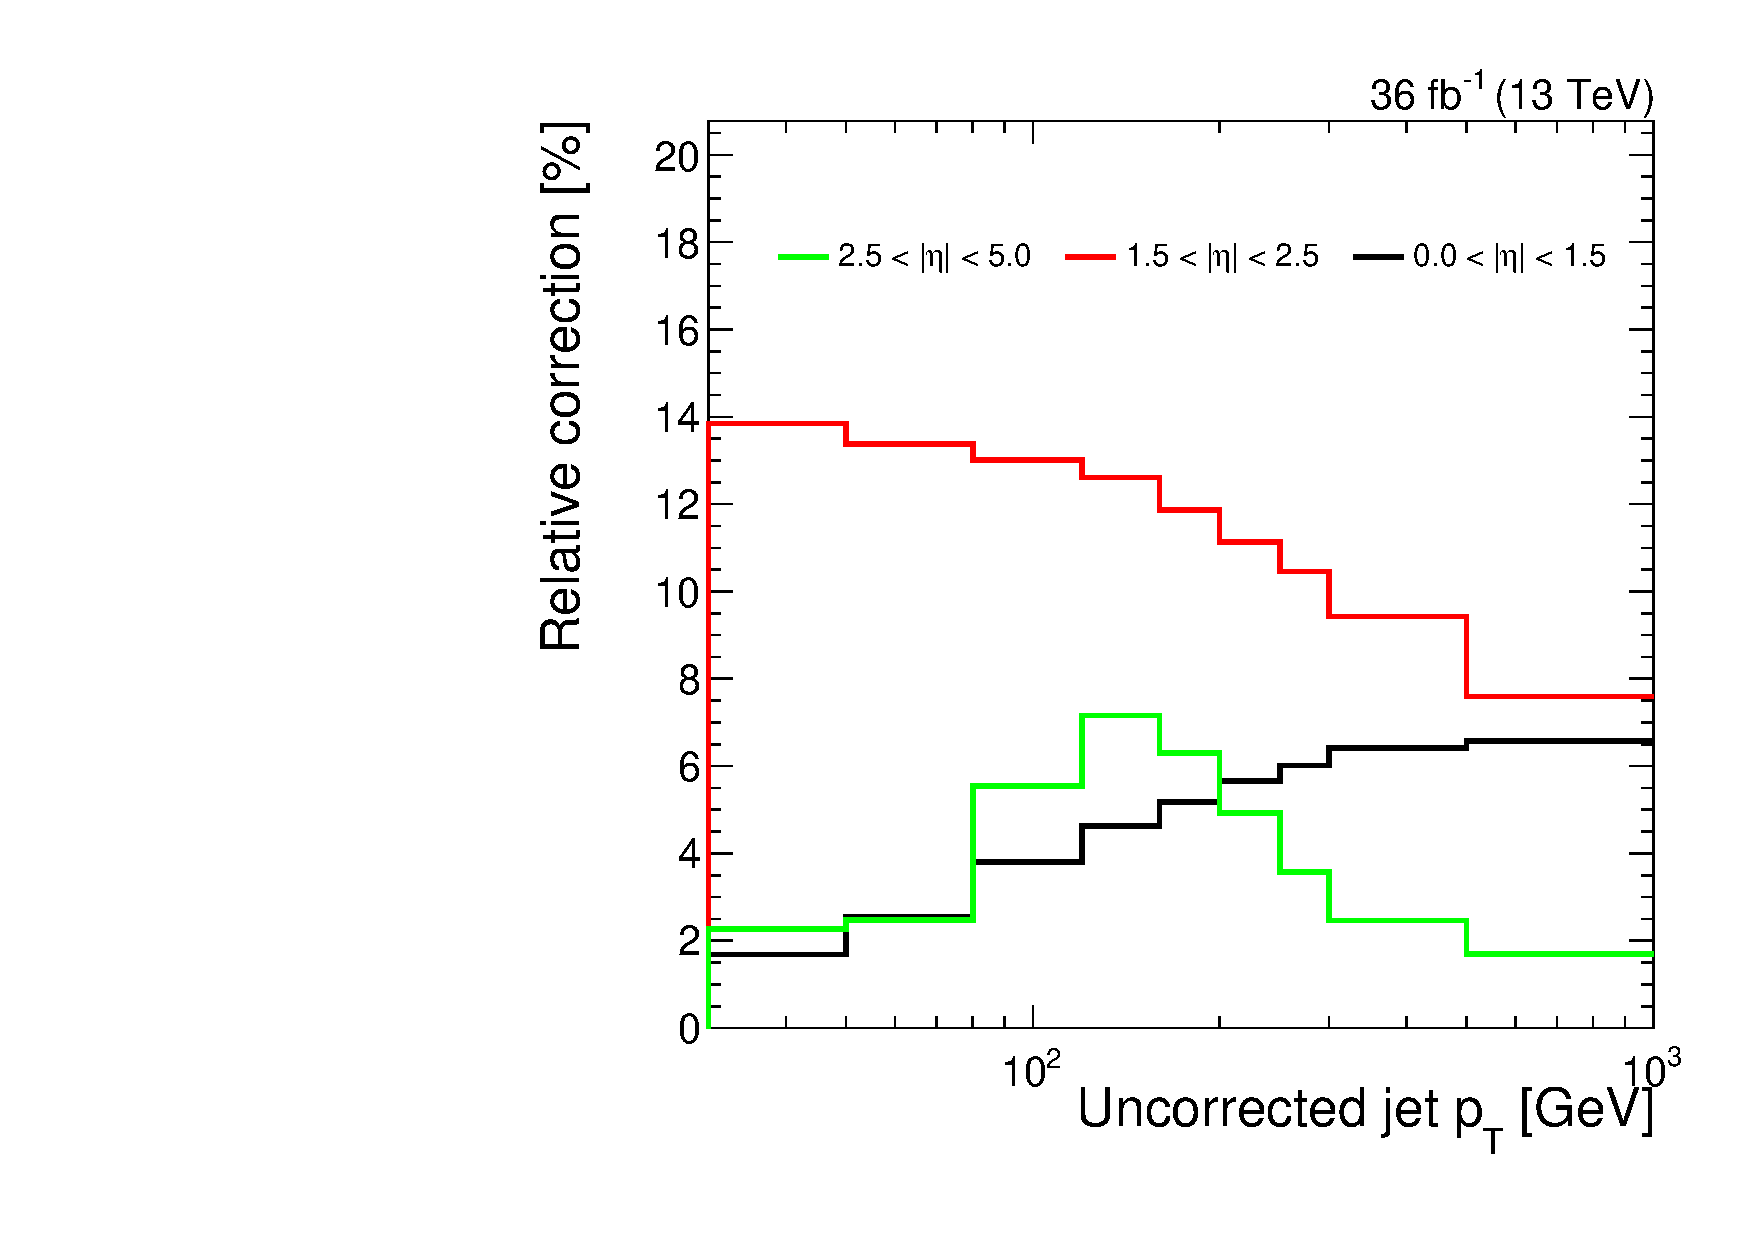
\includegraphics[width=0.35\textwidth]{figures/cms/jec_jotjotRawPt.pdf}
    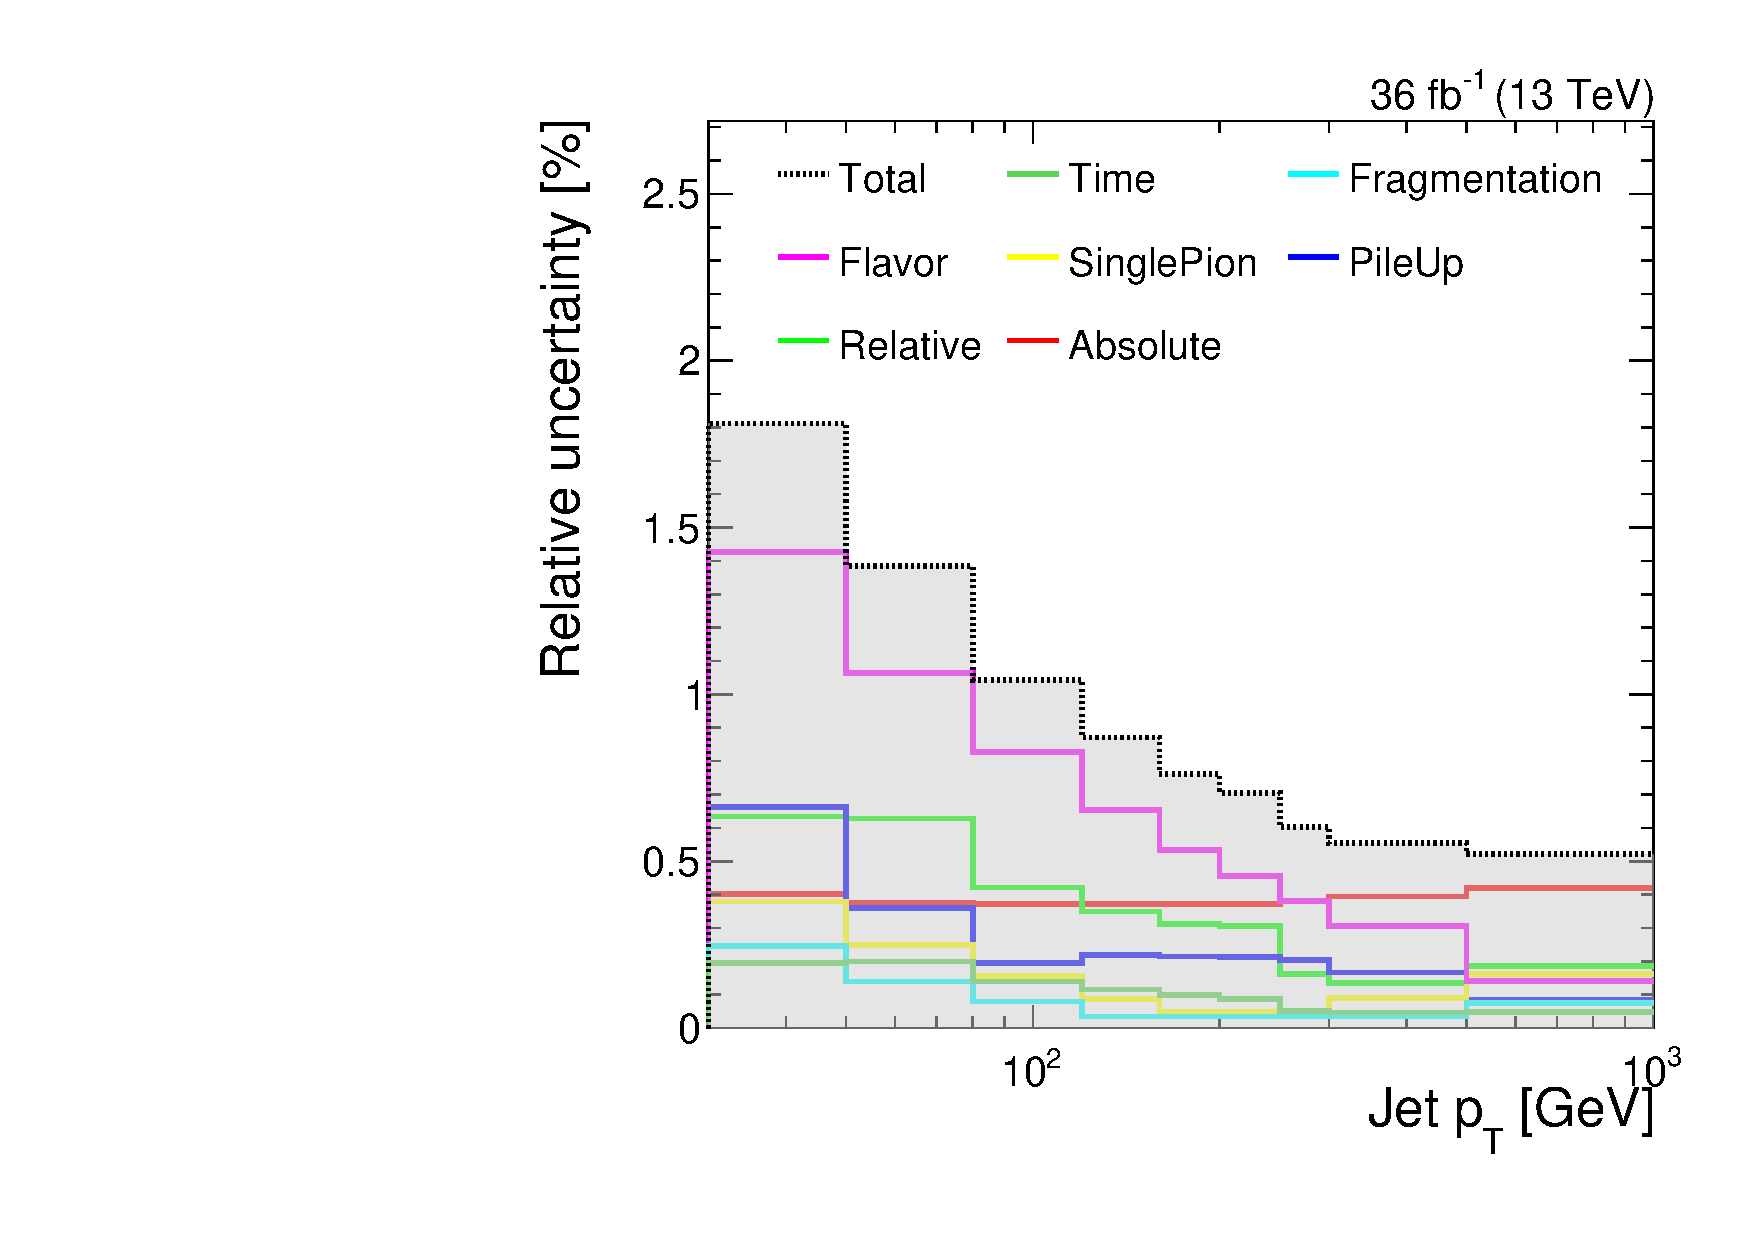
\includegraphics[width=0.35\textwidth]{figures/cms/var_jotjotPt.pdf}
    \caption{Left: the total effect of the L1 and L2L3 jet energy scale corrections in MC, as a function of $\pt,\eta$.
             Right: the corresponding uncertainties on the JES corrections, in the same \pt~binning and averaged over $\eta$.}
    \label{fig:cms:jec}
\end{center}
\end{figure}

\subsubsection{Heavy flavor jet ID}

It is frequently useful to identify the type of parton that induces a jet.
In the context of the results presented in this thesis, identifying $b$ quarks ($b$-tagging) is important, but identifying other initial states is also possible ($c$ quarks, gluons vs quarks). 
The hadronization of a $b$ quark involves the production of a $b$ hadron, which have lifetime of $\tau\sim 1.5$ ps. 
The lab frame displacement is $\gamma\beta c\tau = \nicefrac{pc\tau}{m}$.
A $B$ meson with $\pt=50$ GeV will have a mean transverse displacement of $4.3$ mm, which is well within the vertexing resolution of the pixel detector.
Therefore, the signature of a $b$ jet is the identification of an SV displaced from the PV, with properties consistent with a heavy hadron (Figure~\ref{fig:cms:bjet}).

\begin{figure}[]
\begin{center}
    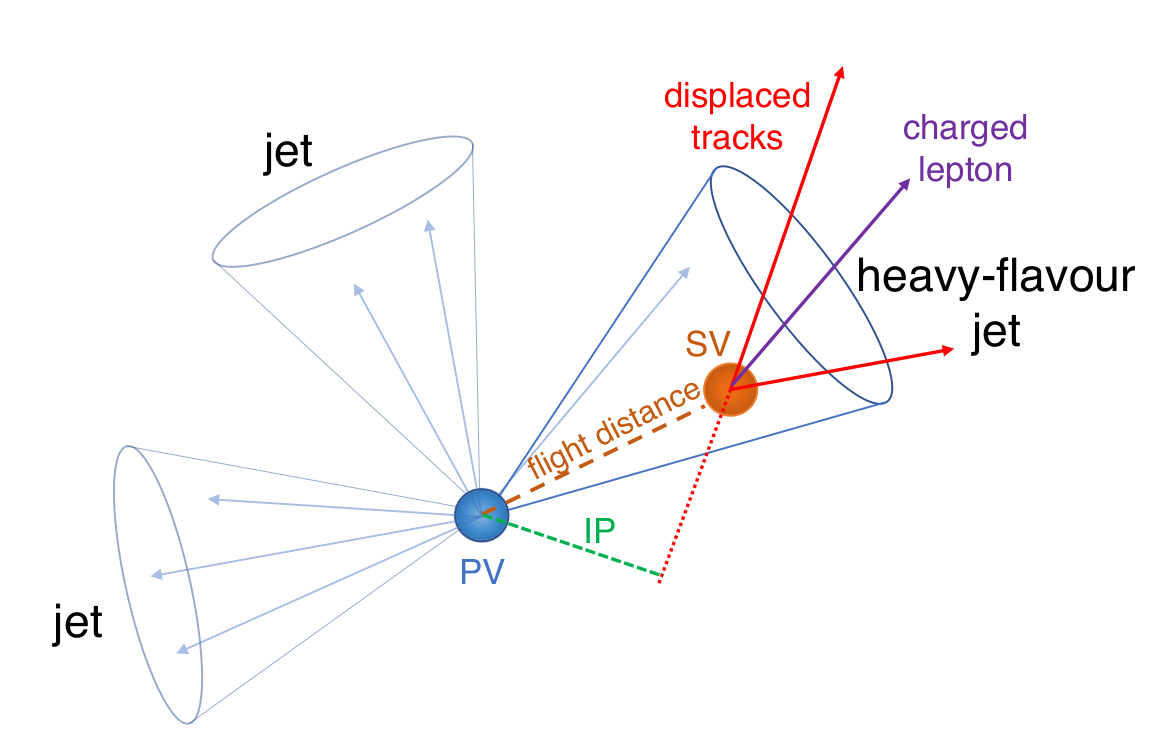
\includegraphics[width=0.5\textwidth]{figures/cms/bjet.png}
    \caption{Location of a secondary vertex inside a $b$ jet.
             Reprinted from Reference~\cite{csvv2}.}
    \label{fig:cms:bjet}
\end{center}
\end{figure}

The reconstruction of the SV is described in Section~\ref{sec:cms:tracker}.
The Combined Secondary Vertex (CSVv2) tagger~\cite{csvv2} is an artificial neural network trained to distinguish $b$ jets from $u/d/c/s/g$ jets. 
Nineteen characteristics of the jet (e.g. mass of tracks associated with the SV, presence of soft leptons from the SV, $d_0$ of the SV) are used to train the NN\footnote{See Section 4.1.2.1 of Reference~\cite{csvv2} for a full list.}.
For the analyses described in this thesis, a jet is considered $b$-tagged if it satisfies CSVv2 $>0.54$. 
Discrepancies between data and MC in the efficiency of the $b$ jet ID are corrected for using SFs, derived separately for $b$ and non-$b$ jets.
Two $b$-enriched samples are used for the former task.
The first is a relatively pure, but statistically limited, sample of $t\bar{t}$ events, in which the $b$ quarks from the $t$ quark decays are used.
The second is a much more statistically powerful sample of $g\rightarrow b\bar{b}$ events, which is selected by triggering on and identifying a non-isolated muon from the decay of one of the $b$ hadrons. 
Figure~\ref{fig:cms:csvv2} compares the CSVv2 response in data and simulation, as well as the SFs used to correct this distribution.

\begin{figure}[]
\begin{center}
    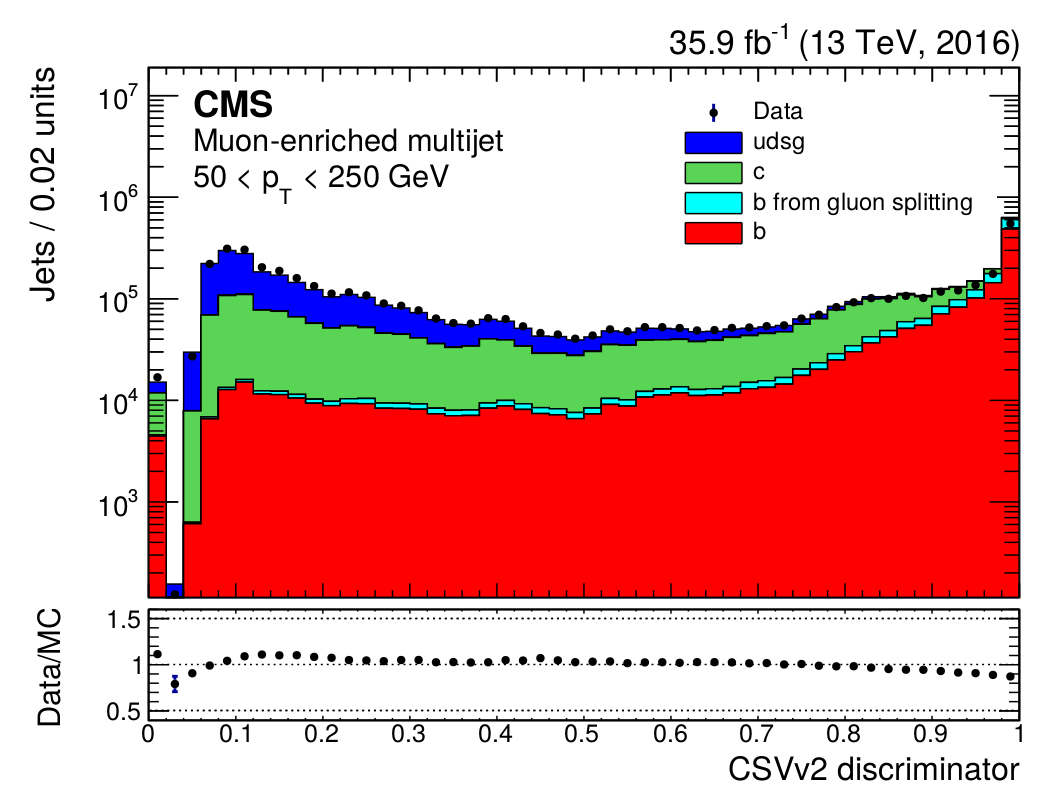
\includegraphics[width=0.48\textwidth]{figures/cms/csvv2.png}
    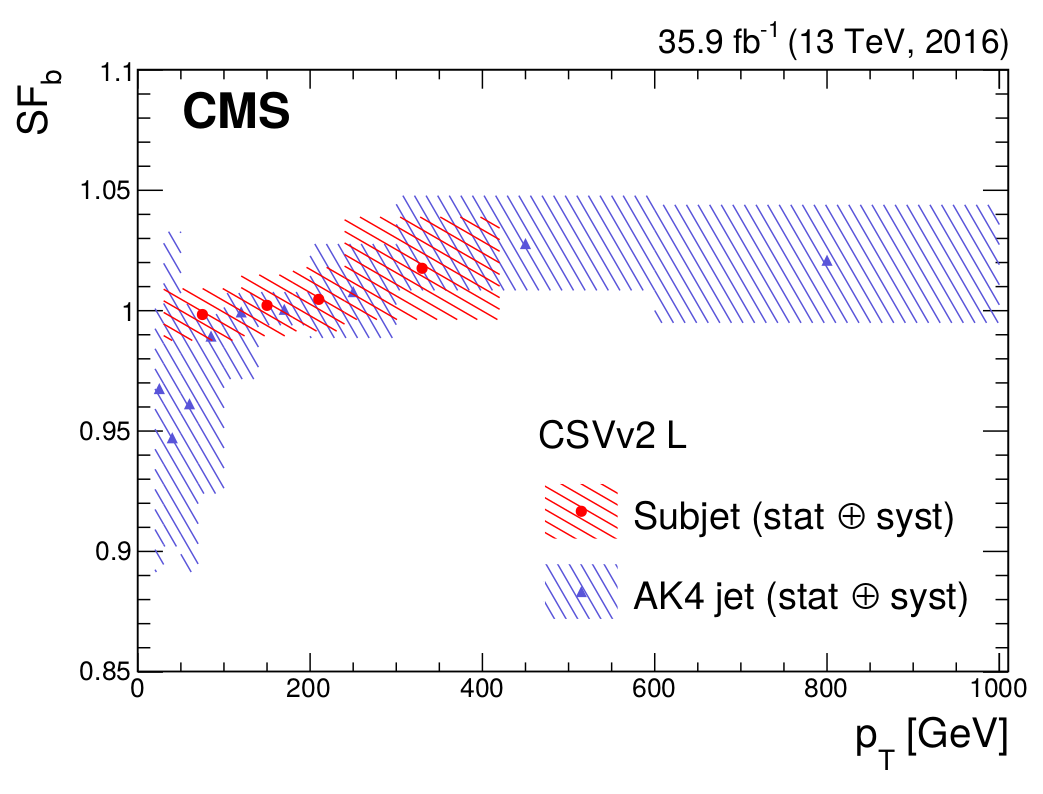
\includegraphics[width=0.48\textwidth]{figures/cms/csvsf.png}
    \caption{Left: The distribution of the CSVv2 response of AK4 jets in a dijet sample enriched with $g\rightarrow b\bar{b}$ events.
             Right: data/MC scale factors to correct for discrepancies in the simulation of the $b$ jet ID.
             AK4 jet SFs and uncertainties are shown in blue; overlaid in red are the SFs for subjets (see Chapter~\ref{sec:jets}).
             Reprinted from Reference~\cite{csvv2}.}
    \label{fig:cms:csvv2}
\end{center}
\end{figure}

\subsection{Hadronic taus}

A hadronic tau ($\tau_h$) is defined as a tau lepton which decays to one $\nu_\tau$ and one or more hadrons.
A dedicated algorithm~\cite{cmspf,tauid} is used to extract $\tau_h$ candidates from the AK4 jet collection.
Only jets within the tracker acceptance and with $\pt>13$ GeV are used.
Combinations of particles within the jet are considered for compatibility with decay modes consisting of a tau neutrino, 0-2 neutral pions, and 1 or 3 charged hadrons.
While other hadronic final states exist, they have a fairly small branching ratio and are not considered.
The $\pi^0$ will present in the jet as two photons; in some cases, a photon may convert into an $e^-e^+$ pair. 
In the case of multi-hadron final states, compatibility with intermediate resonance masses is checked.
The highest \pt~$\tau_h$ candidate in the jet is selected as a PF $\tau_h$.
To reduce the large combinatorial background from quark and gluon jets, stringent requirements are made on the PF isolation.
A true $\tau_h$ should be fairly well-isolated, whereas a combinatorial fake will be surrounded by a parton shower. 

\subsection{Missing momentum}
\label{sec:cms:met}

The PF missing momentum (\ptmiss) is defined as the magnitude of the missing momentum vector:
\begin{equation}
    \vec{p}_\mathrm{T}^\mathrm{~miss} = -\sum_{i\in\,\text{PF cands.}} \left(\begin{matrix} p_x^{(i)} \\ p_y^{(i)} \end{matrix}\right)
\end{equation}
As the initial state has no net transverse momentum, conservation of momentum requires the same to be true of the final state.
In a perfectly reconstructed event, non-zero \ptmiss~implies the presence of non-interacting particles such as neutrinos or DM candidates.

Fake energy reconstruction or failure to properly reconstruct energy deposits can lead to large, fake~\ptmiss.
Such events are removed through a series of filters:
\begin{itemize}
    \item HCAL and ECAL filters, identifying events with calorimeter clusters caused by noise. 
            The shape and timing of the energy distribution can be used to identify noise, as well as detector-specific information (such as known problematic ECAL crystals).
    \item Beam halo filter, identifying energy deposits from muons traveling parallel to the beam. 
          These muons are produced from pre-collision interactions between the beam and the machine.
          They are identified by their localization in $\phi$ and longitudinal signature in the ECAL/CSCs.
    \item Reconstruction filters, identifying failures of the PF algorithm to properly reconstruct particles.
          In some cases, muons can be double-counted or mis-identified as charged hadrons and muons.
\end{itemize}
These filters remove effectively all anomalous \ptmiss~events while rejecting less than 1\% of events with real \ptmiss. 

As the \ptmiss~indirectly depends on the momentum of each PF candidate that enters the sum, any \emph{ad hoc} calibrations must be propagated.
Most energy calibrations are intrinsic to the PF algorithm, but the jet energy scale corrections are not.
Therefore, the missing momentum is accordingly updated:
\begin{equation}
    \vpt{~\mathrm{miss}} \mapsto \vpt{~\mathrm{miss}}  + \sum_{j\in\,\mathrm{jets}} \left(\vpt{~j,\mathrm{corr.}} - \vpt{~j,\mathrm{raw}}\right) 
\end{equation}

\subsection{Pileup mitigation}

Two algorithms are used to mitigate the effects of pileup in jets: charged hadron subtraction (CHS) and pileup per-particle identification (PUPPI)~\cite{puppi}.
CHS simply removes charged particles not from the primary vertex from the set of PF candidates fed into the jet clustering.
This is only able to remove charged pileup contamination for jets within the tracker acceptance.

The PUPPI algorithm defines a local shape $\alpha_i$ for every particle $i$ in the event that is independent of particle location or charge.
The distribution of $\alpha_i$ is determined for central, charged particles from the PV and from PU.
This is then extrapolated to neutral particles and forward particles, to assign a probability $P(\mathrm{PU}|\alpha_i)$. 
More concretely, the local shape is defined:
\begin{equation}
    \alpha_i = \log \sum_{j \neq i} \frac{\ptj}{\Delta R_{ij}} H(\Delta R_{ij} - R_{\min})H(R_0 - \Delta R_{ij})
\end{equation}
where $R_{\min}, R_0$ are tunable parameters and $H$ is the Heaviside step function. 
Up to rescaling, $\alpha_i$ is the sum of \pt s of particles in an annulus around particle $i$. 
It is expected to be larger for PV particles than PU particles, as PU radiation is uniformly distributed, whereas PV radiation is centered around hard partons.
This is illustrated in Figure~\ref{fig:cms:puppi}, which shows $\alpha_i^F$ (same as $\alpha_i$) and $\alpha_i^C$ (same as $\alpha_i$, except sum only charged particles).

\begin{figure}[]
\begin{center}
    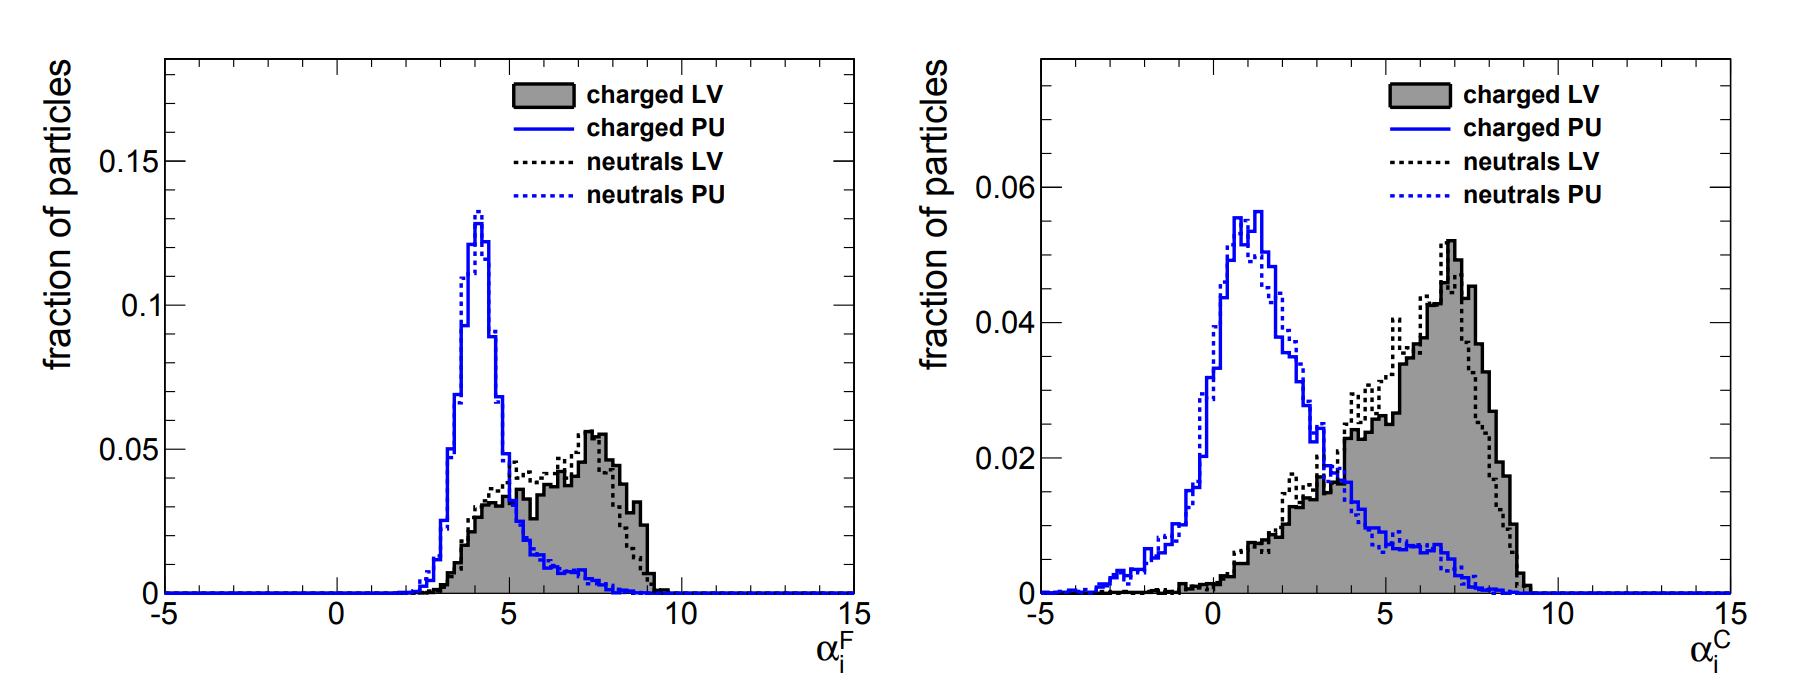
\includegraphics[width=0.8\textwidth]{figures/cms/puppi.png}
    \caption{Distribution of PUPPI local shapes for charged and neutral particles from the PV and PU vertices.
             Reprinted from Reference~\cite{puppi}.}
    \label{fig:cms:puppi}
\end{center}
\end{figure}

Then, we define:
\begin{equation}
    x_i = H(\alpha_i - \bar\alpha) \frac{(\alpha_i - \bar\alpha)^2}{\sigma^2}
\end{equation}
where $\bar\alpha$ and $\sigma$ are the median and RMS, respectively, of the charged PU $\alpha_i$ distribution, with some extrapolation for $\eta_i$ and $q_i$.
It is found that $\alpha_i$ has a Gaussian distribution for pileup, and so $x_i$ should have a $\chi^2$ distribution with 1 degree of freedom.
Therefore, we define the probability of pileup as:
\begin{equation}
w_i = 1 - P(\mathrm{PU}|\alpha_i) = 
    \begin{cases}
        1 & \text{if }|\eta|<2.5,~q_i \neq 0, \text{ from PV} \\ 
        0 & \text{if }|\eta|<2.5,~q_i \neq 0, \text{ not from PV} \\ 
        P(\chi^2<x_i | N_\mathrm{dof}=1)  & \text{otherwise} \\ 
    \end{cases}
\end{equation}
The four momenta of particles are scaled by the PUPPI probability, i.e. $p_i^\mu \mapsto w_i p_i^\mu$.

In the context of the results described in this analysis, it is found that CHS provides sufficient pileup mitigation for AK4 jets, but as described in Chapter~\ref{sec:jets}, PUPPI will be necessary for CA15 jets. 

\section{Simulation of CMS}
\label{sec:cms:sim}

The CMS offline software suite (CMSSW~\cite{cmssw}) uses Geant4 \cite{geant1,geant2} to simulate the detector response to particles produced in collisions. 
As described in Section~\ref{sec:theory}, particle-level MC simulates the hard scattering and  parton shower.
Multiple simulated proton-proton collisions are overlaid into a single event to mimic the effect of pileup. 
The generate particles are then interfaced to Geant4, which simulates the passage of a particle through the magnetic field, the energy deposited as the particle interacts with the detector material, and the evolution of any additional particles produced (e.g. EM showers).
The readout electronics' response to the detector signature is then simulated.
The software used to reconstruct the simulated electronic response is identical to that used for real data.
This minimizes any reconstruction differences between MC and data.
Additional truth information from the generators is retained for use in data analysis tasks.

